\documentclass[a4paper,12pt,twoside,BCOR=10mm]{scrbook}

% IMPORTANT TODO :: go through all TODOs and especially all IMPORTANT TODOs!
%
% for citation commands, see:
% http://merkel.zoneo.net/Latex/natbib.php
%
% Here are the ones that we use; first the two main ones:
% \citep{jon90}               --> (Jones et al., 1990)
% \citep[see][]{jon90}        --> (see Jones et al., 1990)
%
% But we also have for a specific part (chapter, page, ...) that is cited:
% \citep[chap. 2]{jon90}      --> (Jones et al., 1990, chap. 2)
% \citep[see][chap. 2]{jon90} --> (see Jones et al., 1990, chap. 2)
% see \citet[chap. 2]{jon90}  --> see Jones et al. (1990, chap. 2)
%
% And if we want to cite several at once:
% \citep{jon90,jam91}         --> (Jones et al., 1990; James et al. 1991)
%
% Finally, for in-text citations, we have:
% \citet{jon90}               --> Jones et al. (1990)
%
%
%
% TODO :: search for every occurrence of "\color{red}" or of "(imagine some text here)" and figure that stuff out =)
%
% TODO :: das ganze Dokument durchsuchen und "Burrows-Wheeler", "Burrows---Wheeler", "Burrows - Wheeler"
%         durch "Burrows--Wheeler" ersetzen sowie "preprocess" durch "pre-process" ersetzen (oder andersrum,
%         aber jedenfalls nicht andauernd hin und her springen ^^), "bit-vector" durch "bit vector" ersetzen
%         und schließlich auch noch "\cite{" durch "\citep{" sowie "Javascript" durch "JavaScript" (CamelCase, yay! ^^)
%
% TODO :: decide whether to use SNPs or snips, and then stick with one ;) (just now I used "snips", but seriously, check that!)
%
% TODO :: replace " - " with "---" (but case-to-case, nicht einfach so blanko!)
%
% TODO :: replace " we " with " I "? (but case-to-case, nicht einfach so blanko!)
%
% TODO :: alles nochmal auf verb tenses überprüfen, also:
% "Use present tense to express general truths or facts or conclusions supported by research results that are unlikely to change.
% In other words, something that is believed to be always true."
% http://cgi.stanford.edu/~dept-ctl/tomprof/posting.php?ID=1009
%
% TODO :: nochmal durchschauen, ob wir die folgenden Regeln alle so richtig eingehalten haben:
%
% alle Texte sollen schwarz sein (mit Ausnahme von Bildern, in denen auch Farben erlaubt sind)
% fett bitte nur spärlich verwenden
% unterstrichene Texte bitte gar nicht verwenden
% ausdrücklich sollen Hyperlinks vermieden werden, die unterstrichen oder in Farbe dargestellt werden!
% man sollte sparsam mit footnotes (also Fußnoten) umgehen
%   wenn man sie einsetzt, dann sollten sie nummeriert sein und möglichst direkt auf der Seite der ersten Erwähnung aufgeführt werden
% man sollte nicht tiefer als subsubsections gehen, also: chapters ok, sections ok, subsections ok, subsubsections ok, mehr nicht =) 
%
%
% zum Druck:
% 
% alles soll in A4 ausgedruckt werden
% natürlich soll beidseitig gedruckt werden, und Kapitel sollen immer auf der rechten Seite starten
% die Druckerei erwartet oft eine PDF-Datei
% (die meist mit höchstmöglichen qualitativen Einstellungen exportiert werden muss und alle Bilder embedded hat)
% Achtung! Farbdrucke sind nicht gerade billig, hier aber echt notwendig. ;)
%
%
% und noch ein paar Dinge:
%
% Title page, spine, and back page
% 
% Logos of sponsors or whoever should not be used; not on the front, the back, or anywhere else either ;)
% Instead, all thanks should go into a chapter "Acknowledgements" or in the preamble. (And even then as text, not logo!)
% There should be no picture on the front.
% 
% On the backside can be the name of the printing press (at most 10 pt Verdana in regular white letters),
% þá miðjað hægri-vinstri á blaðsíðu og miðjað upp-niður innan litaborðans. 
% 
% The colored area should go around the spine and onto the back of the book, and go 7,7 cm up from the bottom of the page.
% 
% The colored area should be orange, the color of the Natural Sciences at UI.
% In particular, the color is: CMYK:  0 : 75 : 100 : 0; Pantone: 158 C; RGB: 236 : 78 : 34.
% 
% On the spine of the book you should have the name of the author, the short title (no more than 50 characters)
% and the year of publication in one line in Verdana.
% (The year should be in white letters on the colorful background, while the name of the author and the title should be
% black on white.)
% 
% Here are two examples / instructions on how to do things right:
% 
% Friðrík H. Jónsson og Sigurður J. Grétarsson (2007). \textit{Gagnfræðikver fyrir háskólanema}, Háskólaútgáfan, Reykjavík.
% Ingibjörg Axelsdóttir og Þórunn Blöndal (2006).  \textit{Handbók um ritun og frágang},  Mál og menning, Reykjavík.
 
% Packages
\usepackage{ucs}
\usepackage[utf8x]{inputenc}
\usepackage[icelandic, english]{babel}
\usepackage{t1enc}
\usepackage{graphicx}
\usepackage[intoc]{nomencl}
\usepackage{enumerate,color}
\usepackage[hyphens]{url}
\usepackage[pdfborder={0 0 0}]{hyperref}
\usepackage{appendix}
\usepackage{eso-pic}
\usepackage{amsmath}
\usepackage{amssymb}

% we added this one to get numbered definitions and theorems and proofs and so on... not sure if we should even have them,
% as this is compsci, not maths (and in fact it kind of is bioinformatics, so it is even further removed from nice maths ^^),
% but f it - proofs and definitions are a language we speak, and we MAKE IT SO! =)
\usepackage{amsthm}
% this here should be theoremstyle plain for the theorem, but then the theorem is written in italics, and I really want to
% avoid that as I honestly think it is difficult to read...
% \theoremstyle{definition}
% \newtheorem{moyatheorem}{Theorem}[chapter]
% \theoremstyle{definition}
% \newtheorem{moyadef}{Definition}[chapter]

\usepackage[nottoc,numbib]{tocbibind}
\usepackage[sort&compress,authoryear]{natbib}
%\usepackage[sort&compress,square,numbers]{natbib}
\bibliographystyle{abbrvnat}
\setcitestyle{authoryear,open={(},close={)}}

\usepackage[sf,normalsize]{subfigure}
\usepackage[format=plain,labelformat=simple,labelsep=colon]{caption}
\usepackage{placeins}
\usepackage{tabularx}
\usepackage{filecontents}

% following line added based on Pall's email
\usepackage[a4paper,left=3cm,right=2cm,top=2.5cm,bottom=2.0cm, includefoot]{geometry}

% following line added for algorithm environments and to print a list of algorithms;
% see https://en.wikibooks.org/wiki/LaTeX/Algorithms
\usepackage[chapter]{algorithm}
\usepackage{algpseudocode}

% make table of contents clickable (in electronic devices, of course... not on paper ^^)
\usepackage{hyperref}

% BTW, for example reference types, see https://www.sharelatex.com/learn/Bibliography_management_with_natbib

\begin{filecontents*}{thesisreferences.bib}
%
% ===================================================================================================================
%                                                     REFERENCES
% ===================================================================================================================
%
@article{Siren2014,
    author =       "Jouni Sirén and Niko Välimäki and Veli Mäkinen",
    title =        "Indexing Graphs for Path Queries with Applications in Genome Research",
    journal =      "IEEE/ACM Transactions on Computational Biology and Bioinformatics",
    volume =       "11",
    number =       "2",
    pages =        "375--388",
    year =         "2014",
    DOI =          "10.1109/TCBB.2013.2297101"
}
@book{bioinfoalgorithms,
    author    = "Phillip Compeau and Pavel Pevzner",
    title     = "Bioinformatics Algorithms",
    year      = "2014",
    publisher = "Active Learning Publishers",
    address   = "La Jolla, CA, USA",
	ISBN      = "978-0-9903746-0-2"
}
@online{specFASTG,
    author =       "David Jaffe and Iain MacCallum and Daniel Rokhsar and Michael Schatz",
    title =        "The FASTG Format Specification",
    version =      "1.00",
    year =         "2012",
	URL =          "http://fastg.sourceforge.net/FASTG_Spec_v1.00.pdf",
	note =         "Accessed: 4th of April 2015"
}
@online{specGFA1,
    author =       "Heng Li",
	title =        "A proposal of the Grapical Fragment Assembly format",
    year =         "2014",
    URL =          "http://lh3.github.io/2014/07/19/a-proposal-of-the-grapical-fragment-assembly-format/",
	note =         "Accessed: 4th of April 2015"
}
@online{specGFA2,
    author =       "Heng Li",
	title =        "First update on GFA",
    year =         "2014",
    URL =          "http://lh3.github.io/2014/07/23/first-update-on-gfa/",
	note =         "Accessed: 4th of April 2015"
}
@online{specGFA3,
    author =       "Heng Li",
	title =        "On the graphical representation of sequences",
    year =         "2014",
    URL =          "http://lh3.github.io/2014/07/25/on-the-graphical-representation-of-sequences/",
	note =         "Accessed: 5th of April 2015"
}
@online{knightGFA1,
    author =       "James Knight",
	title =        "Graphs, Alignments, Variants and Annotations, pt. 1",
    year =         "2014",
    URL =          "http://knightlab.commons.yale.edu/gava-pt-1/",
	note =         "Accessed: 6th of April 2015"
}
@online{knightGFA2,
    author =       "James Knight",
	title =        "Graphs, Alignments, Variants and Annotations, pt. 2",
    year =         "2014",
    URL =          "http://knightlab.commons.yale.edu/gava-pt-2/",
	note =         "Accessed: 6th of April 2015"
}
@online{specSAM,
    author =       "{The SAM/BAM Format Specification Working Group}",
    title =        "Sequence Alignment/Map Format Specification",
    version =      "ec1fec2",
    year =         "2015",
	URL =          "http://samtools.github.io/hts-specs/SAMv1.pdf",
	note =         "Accessed: 23rd of April 2015"
}
% SAM2009 is reference [4] from the grant proposal.
@article{SAM2009,
    author =       "Heng Li and Bob Handsaker and Alec Wysoker and Tim Fennell and Jue Ruan and Nils Homer and Gabor Marth and Goncalo Abecasis and Richard Durbin and 1000 Genome Project Data Processing Subgroup",
    title =        "The Sequence Alignment/Map format and SAMtools",
    journal =      "Bioinformatics",
    volume =       "25",
    number =       "16",
    pages =        "2078--2079",
    year =         "2009",
    DOI =          "10.1093/bioinformatics/btp352"
}
% in this paper, BWA is explained
@article{Li2009,
    author =       "Heng Li and Richard Durbin",
    title =        "Fast and accurate short read alignment with Burrows--Wheeler transform",
    journal =      "Bioinformatics",
    volume =       "25",
    number =       "14",
    pages =        "1754--1760",
    year =         "2009",
    DOI =          "10.1093/bioinformatics/btp324"
}
% in this paper, BWA-MEM is explained
@article{Li2013,
    author =       "Heng Li",
    title =        "Aligning sequence reads, clone sequences and assembly contigs with BWA-MEM",
    year =         "2013",
    note =         "arXiv:1303.3997 [q-bio.GN]"
}
% Burrows1994 is reference [5] from Siren2014.
% It is the paper in which the BWT was introduced; not having anything to do with bioinformatics, mind you,
% but as a compression algorithm!
@online{Burrows1994,
    author =       "Michael Burrows and David J. Wheeler",
	title =        "A block-sorting lossless data compression algorithm. \textit{Digital Equipment Corporation.} Tech. Rep. 124",
    year =         "1994",
    URL =          "http://www.hpl.hp.com/techreports/Compaq-DEC/SRC-RR-124.html",
	note =         "Accessed: 7th of April 2015"
}
% Schneeberger2009 is reference [12] from Siren2014.
% Gives the much-needed basis for the hash-based approach.
% In general, it is very full of awesome ideas and approaches, both in its intro and outro and everywhere in between. =D
@article{Schneeberger2009,
    author =       "Korbinian Schneeberger and Jörg Hagmann and Stephan Ossowski and Norman Warthmann and Sandra Gesing and Oliver Kohlbacher and Detlef Weigel",
    title =        "Simultaneous alignment of short reads against multiple genomes",
    journal =      "Genome Biology",
    volume =       "10",
    number =       "9",
    pages =        "R98",
    year =         "2009",
    DOI =          "10.1186/gb-2009-10-9-r98"
}
% Puglisi2007 is reference [21] from Siren2014.
@article{Puglisi2007,
    author =       "Simon Puglisi and W. F. Smyth and Andrew H. Turpin",
    title =        "A Taxonomy of Suffix Array Construction Algorithms",
    journal =      "ACM Computing Surveys",
    volume =       "39",
    number =       "2",
    pages =        "Article 4",
    year =         "2007",
    DOI =          "10.1145/1242471.1242472"
}
% Albers2010 is reference [13] from Siren2014.
@article{Albers2010,
    author =       "Cornelis A. Albers and Gerton Lunter and Daniel G. MacArthur and Gilean McVean and Willem H. Ouwehand and Richard Durbin",
    title =        "Dindel: Accurate indel calls from short-read data",
    journal =      "Genome Research",
    volume =       "21",
    pages =        "961--973",
    year =         "2011",
    DOI =          "10.1101/gr.112326.110"
}
% Huang2013 is reference [14] from Siren2014.
@article{Huang2013,
    author =       "Lin Huang and Victoria Popic and Serafim Batzoglou",
    title =        "Short read alignment with populations of genomes",
    journal =      "Bioinformatics",
    volume =       "29",
    number =       "13",
    pages =        "i361--i370",
    year =         "2013",
    DOI =          "10.1093/bioinformatics/btt215"
}
@article{Lee2002,
    author =       "Christopher Lee and Catherine Grasso and Mark F. Sharlow",
    title =        "Multiple sequence alignment using partial order graphs",
    journal =      "Bioinformatics",
    volume =       "18",
    number =       "3",
    pages =        "452--464",
    year =         "2002",
    DOI =          "10.1093/bioinformatics/18.3.452"
}
@article{Holt2014,
    author =       "James Holt and Leonard McMillan",
    title =        "Constructing Burrows--Wheeler Transforms of Large String Collections via Merging",
    journal =      "BCB '14, Proceedings of the 5th ACM Conference on Bioinformatics, Computational Biology, and Health Informatics",
    pages =        "464--471",
    year =         "2014",
    DOI =          "10.1145/2649387.2649431"
}
% Myers 2005 seems to be mostly about DNA string graphs (yay!) used when building up a NEW unknown reference 
% from reads only, not for aligning reads to an already existing reference...
% But still, it looks like it can be helpful and citeable! =)
@article{Myers2005,
    author =       "Eugene W. Myers",
    title =        "The fragment assembly string graph",
    journal =      "Bioinformatics",
    volume =       "21",
    number =       "Suppl. 2",
    pages =        "ii79--ii85",
    year =         "2005",
    DOI =          "10.1093/bioinformatics/bti1114"
}
@online{Li2014,
    author =       "Heng Li",
	title =        "Experimenting FM-index for multiple human samples",
    year =         "2014",
    URL =          "http://files.figshare.com/1614096/HengLi_20140717.pdf",
	note =         "Accessed: 6th of April 2015"
}
% Makinen2010 is reference [11] from Siren2014.
@article{Makinen2010,
    author =       "Veli Mäkinen and Gonzalo Navarro and Jouni Sirén and Niko Välimäki",
    title =        "Storage and Retrieval of Highly Repetitive Sequence Collections",
    journal =      "Journal of Computational Biology",
    volume =       "17",
    number =       "3",
    pages =        "281--308",
    year =         "2010",
    DOI =          "10.1089/cmb.2009.0169"
}
% Navarro2007 is reference [6] from Siren2014.
@article{Navarro2007,
    author =       "Gonzalo Navarro and Veli Mäkinen",
    title =        "Compressed full-text indexes",
    journal =      "ACM Computing Surveys",
    volume =       "39",
    number =       "1",
    pages =        "Article 2",
    year =         "2007",
    DOI =          "10.1145/1216370.1216372"
}
% Ferragina2009 is reference [10] from Siren2014.
@article{Ferragina2009,
    author =       "Paolo Ferragina and Fabrizo Luccio and Giovanni Manzini and S. Muthukrishnan",
    title =        "Compressing and indexing labeled trees, with applications",
    journal =      "Journal of the ACM",
    volume =       "57",
    number =       "1",
    pages =        "Article 4",
    year =         "2009",
    DOI =          "10.1145/1613676.1613680"
}
% Langmead2009 is reference [2] from the grant proposal.
@article{Langmead2009,
    author =       "Ben Langmead and Cole Trapnell and Mihai Pop and Steven L. Salzberg",
    title =        "Ultrafast and memory-efficient alignment of short DNA sequences to the human genome",
    journal =      "Genome Biology",
    volume =       "10",
    number =       "3",
    pages =        "R25",
    year =         "2009",
    DOI =          "10.1186/gb-2009-10-3-r25"
}
% McKenna2010 is reference [3] from the grant proposal.
@article{McKenna2010,
    author =       "Aaron McKenna and Matthew Hanna and Eric Banks and Andrey Sivachenko and Kristian Cibulskis and Andrew Kernytsky and Kiran Garimella and David Altshuler and Stacey Gabriel and Mark Daly and Mark A. DePristo",
    title =        "The Genome Analysis Toolkit: A MapReduce framework for analyzing next-generation DNA sequencing data",
    journal =      "Genome Research",
    volume =       "20",
    number =       "9",
    pages =        "1297--1303",
    year =         "2010",
    DOI =          "10.1101/gr.107524.110"
}
% Garrison2012 is reference [5] from the grant proposal.
@article{Garrison2012,
    author =       "Erik Garrison and Gabor Marth",
    title =        "Haplotype-based variant detection from short-read sequencing",
    year =         "2012",
    note =         "arXiv:1207.3907 [q-bio.GN]"
}
% I randomly stumbled over this on twitter... because, oink, why not! =)
% (It may as well apply to our scripts, but not so much to the Delphi MCC because Delphi is not very Linux-y...)
@online{MANIFESTO,
	author =       "Pjotr Prins",
	title =        "Small tools MANIFESTO for Bioinformatics",
	month =        "Feb.",
	year =         "2014",
	URL =          "https://github.com/pjotrp/bioinformatics/blob/master/README.md",
	note =         "Accessed: 27th of July 2015. doi: 10.5281/zenodo.11321"
}
@online{RedditSwitchTo38,
	author =       "Gregory M. Cooper",
	title =        "Switch from hg19/build37 to hg20/build38?",
	year =         "2015",
	URL =          "http://www.reddit.com/r/genome/comments/3b3s3t/switch_from_hg19build37_to_hg20build38/",
	note =         "Accessed: 27th of July 2015"
}
@article{Taivalsaari2008,
    author =       "Antero Taivalsaari and Tommi Mikkonen and Dan Ingalls and Krzysztof Palacz",
    title =        "Web browser as an application platform: the lively Kernel experience",
    year =         "2008",
    note =         "Technical Report, SMLI TR-2008-175, Sun Microsystems"
}
\end{filecontents*}

% Configurations
\graphicspath{{figs/}}
\AtBeginDocument{\renewcommand{\bibname}{References}}

\setlength{\parskip}{\baselineskip}
\setlength{\parindent}{0cm}
\raggedbottom
% \setkomafont{subsection}{\normalfont\sffamily}

% Eins og templatið á að vera
% \setkomafont{captionlabel}{\itshape}
% \setkomafont{caption}{\itshape}

% Mun fallegri lausn
\setkomafont{captionlabel}{\itshape}
\setkomafont{caption}{\itshape}
\setkomafont{section}{\FloatBarrier\Large}
\setcapwidth[l]{\textwidth}
\setcapindent{1em}


% Times new roman
%\usepackage[T1]{fontenc}
%\usepackage{mathptmx}

%%%%%%%%%%% MODIFY THESE LINES ONLY %%%%%%%%%%%%%%%%%%%%%%%%%%%%%%%%%%%%%%%%%%%%%%%%%%%%%%%%%
\def\thesisyear{2016}       					% Year thesis submitted
\def\thesismonth{January}						% Month thesis submitted
\def\thesisauthor{Tom Willy Schiller}			% Thesis authoreiningaraðferðinni
\def\thesistitle{Reference Graph Construction and Merging for Human DNA}	% TODO :: Check if title of thesis still has something
%                                                                                     to do with what we actually ended up doing
\def\thesistitlelineone{Reference Graph Construction}	% Front page title of thesis (line one)
\def\thesistitlelinetwo{and Merging for Human DNA}	% Front page title of thesis (line two)
\def\thesisshorttitle{Reference Graphs for Human DNA} 	% Short title of thesis (50 characters including spaces)
\def\thesiscredits{60} 							% Credits awarded for the project
\def\thesissubject{Computer Science}			% Thesis subject
\def\thesiskind{M.Sc.}							% Masters of PhD thesis
\def\thesiskindformal{Magister Scientiarum}		% Masters of PhD thesis
\def\thesisnroftutors{1}						% Number of tutors
\def\thesisschool{School of Engineering and {Natural Sciences}}		% School
\def\thesisfaculty{Industrial Engineering, Mechanical Engineering and Computer Science}	% Faculty
\def\thesisfacultybroken{Industrial Engineering,\\Mechanical Engineering and Computer Science} % I added this -
%                                                                                                Faculty but broken at a nice place
\def\thesisaddress{VR-II, Hjarðarhaga 2-6}		% TODO :: Office address: Tæknigarður, Dunhagi 5 or VR-II, Hjarðarhaga 2-6
%                                                         depending on who to trust... (both from hi.is)
\def\thesispostalcode{107 Reykjavík}			% Office address
\def\thesistelephone{+354 525 4000}					% Office telephone
\def\thesispublisher{XX}						% (Publisher, not in use)
\def\thesistutors{Páll Melsted \\ (imagine some text here)}					% TODO :: Fill in advisors
\def\thesisrepresentative{(imagine some text here)}				% TODO :: Fill in representative
\def\thesiscommittee{XXNN4 \\ XXNN5}			% (Committee name, not in use)
\def\thesiskeywords{genome sequencing, pan-genome indexing, read alignment, Burrows-Wheeler transform, graph indexing}		% TODO :: Read over keywords and make sure they actually correspond to what we are doing here
\def\thesisdedication{“And above all, watch with glittering eyes the whole world around you,\\
because the greatest secrets are always hidden in the most unlikely places.\\
Those who don't believe in magic will never find it.”\\
–- Roald Dahl}
\def\thesisPrinting{Háskólaprent, Fálkagata 2, 107 Reykjavík}

% Function to add footer to frontpage
\newcommand\BackgroundPic{
\put(0,0){
\parbox[b][\paperheight]{\paperwidth}{
\vfill
\centering
\hspace*{-0.42cm}

\includegraphics[width=\paperwidth,height=\paperheight,
keepaspectratio]{evo_hi_footer.png}
}}
\setlength{\unitlength}{\paperwidth}
\hspace*{-0.3cm}
\begin{picture}(0,0)(0.002,-0.15)
\put(0,0){\color{white}\parbox{1\paperwidth}{\centering\bfseries\sffamily \Large Faculty of \thesisfacultybroken \\
University of Iceland\\
\thesisyear}}
\end{picture}
}

\def\pipe{\texttt{|}}

\begin{document}

\begin{titlepage}
\thispagestyle{empty}
% \AddToShipoutPicture*{\BackgroundPic}
%
\begin{center}
\vspace*{1cm}
\hspace*{-1cm}
%\hspace*{0.6cm}

\includegraphics[width=43.6mm]{evo_ui_logo.png}\\
\vspace*{3.0cm}
\hspace*{-1.05cm}
%\hspace*{0.58cm} % TODO this is the hacked-together title on the title page -
%                       so check if the current title is actually still the same
\huge \sffamily \bfseries \thesistitlelineone \\
\hspace*{-1.25cm}
%\hspace*{0.58cm}
\huge \sffamily \bfseries \thesistitlelinetwo

\vspace*{5.5cm}
\hspace*{-1.35cm}
%\hspace*{0.25cm}
\normalfont \Large \sffamily \thesisauthor
\AddToShipoutPicture*{\BackgroundPic}
\vfill

\end{center}

\newpage 
\thispagestyle{empty} \mbox{}
\newpage
\vspace*{1.35cm}
\thispagestyle{empty}
\begin{center}

\Large \textbf{\sffamily{\MakeUppercase{\thesistitlelineone}}} \\
\Large \textbf{\sffamily{\MakeUppercase{\thesistitlelinetwo}}} \\

\vspace*{1.7cm}
\sffamily{\thesisauthor} \\
\vspace*{1.8cm}
\normalsize \thesiscredits~ECTS thesis submitted in partial fulfillment of a \\
\textit{\thesiskindformal} degree in \thesissubject

\vspace*{1.0cm}
\large
Advisors \\ \thesistutors \\ \vspace*{1.04cm}

Faculty Representative \\
\thesisrepresentative

\vspace*{0.4cm}
\phantom{M.Sc. committee} ~\\
% TODO :: if you want the thesis committee, then replace this by \thesiscommittee with \
% (oh, and the ~\\ in the previous line then should also be a \\ without tilde)
\phantom{thesiscommittee }

\vfill
Faculty of \thesisfacultybroken \\
\thesisschool \\
University of Iceland \\
Reykjavik, \thesismonth~\thesisyear
\newpage
\end{center}
 \newpage
 \thispagestyle{empty}
 \mbox{} \vfill
 % \setcounter{page}{0} \renewcommand{\baselinestretch}{1.5}\normalsize
 \sffamily{\thesistitle} \\
 \sffamily{\thesisshorttitle} \\ % TODO :: maybe take the shorttitle out here if I have shorttitle == longtitle
 \thesiscredits ~ECTS thesis submitted in partial fulfillment of a \thesiskind~degree in \thesissubject
\\ \\
Copyright \textcopyright~\thesisyear~ \thesisauthor \\
All rights reserved \\


Faculty of \thesisfaculty \\
\thesisschool \\
University of Iceland \\
\thesisaddress \\
\thesispostalcode \\
Iceland

Telephone: \thesistelephone \\ \\
\vspace*{\lineskip}

Bibliographic information: \\
\thesisauthor, \thesisyear, \thesistitle, \thesiskind~thesis, Faculty of \thesisfaculty, University of Iceland. \\

Printing: \thesisPrinting \\
Reykjavik, Iceland, \thesismonth~\thesisyear \\
\newpage
\thispagestyle{empty} \mbox{}
\vfill
\begin{center}\textit{\thesisdedication}\end{center} \vspace*{5cm}
\vfill 

\thispagestyle{empty}
\cleardoublepage
\end{titlepage}


% \dedication{\textit{Dedication} \small \\ Tileinkun má sleppa og skal þá fjarlægja blaðsíðuna. \\
% Tileinkun skal birtast á oddatölu blaðsíðu (hægri síðu).}
\pagenumbering{roman}

\setcounter{page}{5}
\section*{\huge Abstract}

% TODO :: Útdráttur á ensku sem er að hámarki 250 orð (currently, I have 161 words).
%         NICHT VERGESSEN! Englische und Isländische Abstracts müssen immer den gleichen Inhalt haben!

The focus of this thesis lies on the computational challenges faced when reading out human DNA. 
In particular, reads of the DNA are commonly aligned with the help of a reference string. 
In this thesis, the opportunities and difficulties of using a graph reference are explored instead. \\
Several approaches for using graph references have already been proposed, 
but none of them are used widely in the field. 
In this thesis the existing approaches are therefore compared and 
new algorithms are developed which are intended to help spread 
the usage of graph references further. 
These algorithms are then collected into the Graph Merging Library GML, 
which can be used to visualize their behaviour to further the understanding 
of these methods. 
In addition to being used for the alignment of reads to reference graphs, 
genomic graphs can also arise in other situations. 
The newly implemented algorithms are general enough to also be of use in these scenarios. \\
Overall, this thesis constitutes a step in the direction of adopting 
the more complicated but also more powerful graphs rather than the sequential string data 
within the field of DNA analysis.

\vspace*{1cm}
\section*{\huge Útdráttur}

% TODO :: Hér kemur útdráttur á íslensku sem er að hámarki 250 orð.
%         Reynið að koma útdráttum á eina blaðsíðu en ef tvær blaðsíður 
%         eru nauðsynlegar á seinni blaðsíða útdráttar að hefjast á oddatölusíðu (hægri síðu).
%         NICHT VERGESSEN! Englische und Isländische Abstracts müssen immer den gleichen Inhalt haben!

(imagine some text here)

\newpage

% \chapter*{Preface}
%
% TODO :: check this makes sense for us
%
% At HÍ, the preface can be left out completely.
% In general, a preface describes the student's role in the work as presented.
% A preface could consist of just one or two sentences.
% Each write-up is tightly focussed on expressing who did what.
%
% For more information, see:
% D:\evo-devo\documents\templates\thesis_sample_prefaces.pdf
%
%
% This thesis is original, unpublished, independent work by the author, \thesisauthor.

\tableofcontents
\listoffigures
\listoftables
\listofalgorithms
\addcontentsline{toc}{chapter}{List of Algorithms}
% TODO :: check if the previous line still works (it add the "List of Algorithms" as entry to the main tableofcontents, 
% but it does it AFTER that page, so basically as long as the list of algorithms fills less than one whole page everything is peachy,
% but if we end up with several hundred algorithms and spill over the page, then the page displayed in the main table of contents
% will probably be wrong

\chapter*{Glossary}
\markboth{GLOSSARY}{}
\addcontentsline{toc}{chapter}{Glossary}

% ====================================================================================================================================
%                                                                                                                             GLOSSARY
% ====================================================================================================================================

% TODO :: hier nochmal drüber schauen und sehen, ob wir noch irgendwelche Erklärungen verbessern können,
%         oder noch irgendwelche Begriffe hinzufügen sollten

% TODO :: check if this format as invisible table is actually really okay with everyone...
%         I mean, it looks rad, but maybe it is not official enough?

% TODO :: measure once more if the final table width is exactly the width of text on the page,
%         I don't want this table here to have drastically different margins
%         (to do this just add a lot of continuous text before the table and see if with the
%         current right paragraph width it ends at the exact same margin on the right side)

% TODO :: Check if all the stuff here is arranged alphabetically.
%         I want it to be alphabetically, so I will start it alphabetically,
%         and it would look really weird to have it nearly-but-not-quite-alphabetically.
%         so yeah, just look over it one more time. ;)

% Í þessum kafla mega koma fram listar yfir skammstafanir og/eða breytuheiti. 
% Gefið kaflanum nafn við hæfi, t.d. Skammstafanir eða Breytuheiti. Þessum kafla má sleppa ef hans er ekki þörf. \\
% The section could be titled: Abbreviations, Glossary, Variable Names, etc.

\begin{tabular}{r p{12cm}}

% TODO :: maybe also add the following:
% edits
% FASTA / FASTQ / GFA / STPU; for each of these, send the reader to the Implementation chapter, Data Formats section
% de novo assembly :: assembly without a reference https://en.wikipedia.org/wiki/De_novo_transcriptome_assembly
% lf-mapping :: last-to-front-mapping or last-to-first-mapping (meaning that the relative positions in the BWT column and in the first column conincide)

\textbf{bps: } &
The pairwise occurring essential building blocks of DNA are referred to as \textit{basepairs.}
% TODO :: actually use this abbreviation somewhere in the text... I think the text that used it has been taken out lol ^^ roflderhatlolgesagt
\\ \\

\textbf{bubble: } &
A \textit{bubble} refers to short alternative paths in a genomic graph, such as 
A[C,G]T, which refers to both ACT and AGT. 
We sometimes wish for data formats to enable a simple inclusion of small \textit{bubbles} without 
the explicit generation of nodes and edges for them, 
as that would lead to a lot of overhead and decrease human-readability, 
while the opposite is also often wished for,
to simplify algorithmically working with the format \citep{specGFA1}.
\\ \\

\textbf{BWT: } &
The \textit{Burrows--Wheeler Transform} is a string compression technique \citep{Burrows1994} 
which is used during the read alignment. For a good introduction to the usage of the BWT 
in bioinformatics, see \citet[chapter 7]{bioinfoalgorithms}.
\\ \\

\textbf{CIGAR: } & 
The \textit{CIGAR string} is a sequence of lengths and operations 
associated with these lengths that is used when aligning one string to another. 
Commonly, they contain the operations \texttt{M} for direct match/mismatch, 
\texttt{I} for insertions and \texttt{D} for deletions. 
However, many additional operations for skipping bases, 
clipping, padding and much more have been proposed 
for various projects \citep{specGFA1,SAM2009,specSAM}.
\\ \\
% a really, REALLY good explanation for CIGAR strings (that I can sadly not quote as it is "just some random wiki":
% http://genome.sph.umich.edu/wiki/SAM#What_is_a_CIGAR.3F
% however, the thing that I actually am citing here (the SAM specification) is at least not too bad either,
% as it nicely defines how the CIGAR is built up

\textbf{indel: } & 
\textit{Insertions} and \textit{deletions} are referred to as \textit{indels}. While 
edit operations merely locally change a character within a string, an insertion or 
deletion affects the index of all the following characters, which is why indels 
usually require more effort to be accurately taken into account.
\\ \\

$k$\textbf{-mer:} &
A nucleotide sequence of length $ k $.
\\ \\

\end{tabular}

\begin{tabular}{r p{12cm}}

\textbf{pipeline: } & 
The \textit{analysis pipeline} refers to any set of programs 
that are used sequentially to reconstruct the full genetic information 
of the individual whose DNA was read out based on a vast amount of short reads and a 
known reference, or to create a list of differences between the individual's DNA 
and the reference.
\\ \\

\textbf{read: } & 
An individual's DNA is often not read out as one continuous string, 
but as large amount of short pieces of DNA. 
These short pieces are referred to as individual \textit{reads.}
\\ \\

\textbf{run-length encoding:} &
A simple method for encoding sequential data by replacing any runs of several 
identical elements with an integer counting the amount of identical elements and 
just one of the elements.
\\ \\

\textbf{self-index:} & 
A \textit{self-index} is a data structure that 
stores sequential data in a compressed form, enables the retrieval of any part of that data without needing 
to access the original data at all, 
and allows efficient pattern searches to be able to quickly perform typical work on the contained data.
\\ \\

\textbf{snip:} &
A \textit{single nucleotide polymorphisms} is a change of a single nucleotide. 
Snips are rather straightforward to work with, as the location of the surrounding data is not affected.
\\ \\

\textbf{variant calling:} & 
The process of finding all nucleotide differences 
between an individual's DNA and a reference. The differences or \textit{variants} are usually reported as positions 
within the reference, and are often given together with confidence estimates.
% TODO :: find a reference for this! (we got it from VariantCallingLecture.pdf in D:, but that is not a good enough source)
\\ \\

\end{tabular}

\chapter*{Acknowledgments}
\addcontentsline{toc}{chapter}{Acknowledgments}

% ====================================================================================================================================
%                                                                                                                      ACKNOWLEDGMENTS
% ====================================================================================================================================

% TODO :: das hier könnte man auch nochmal überarbeiten
%
% Í þessum kafla koma fram þakkir til þeirra sem hafa styrkt rannsóknina með fjárframlögum, aðstöðu eða vinnu. 
% T.d. styrktarsjóðir, fyrirtæki, leiðbeinendur, og aðrir aðilar sem hafa á einhvern hátt aðstoðað við gerð verkefnisins, 
% þ.m.t. vinir og fjölskylda ef við á. Þakkir byrja á oddatölusíðu (hægri síðu).
%
%
% Examples:
%
% Many thanks to all that assisted me throughout the completion of this work, 
% including my supervisor and own professors at the University of Iceland. 
% Without their time, encouragement and support, such a project would not have been possible.
% 
% I would like to thank Ragnar Sigurðsson and Jan Valdman for their guidance and
% support and Fjóla Jónsdottir for insightful comments. I also would like to thank
% Simon Klüpfel for fruitful discussions. Finally I would like to thank my family and
% friends, especially Ragnheiður Einarsdóttir, for their support and patience.
% Thank you.

I would like to thank my tutor, Páll Melsted, for his guidance, support and advice. 
I also would like to thank Mareva Nardelli, Kristinn Ólafsson and Rosemary Milton 
for inspiring me to continue working even when facing difficult problems. 
Finally I would like to thank my family for their ongoing support and curiosity.

Thank you all.

\chapter{Introduction}
\pagenumbering{arabic}
\setcounter{page}{1}

% ====================================================================================================================================
%                                                                                                                         INTRODUCTION
% ====================================================================================================================================

The aim of this thesis is to help improve current approaches from the field of human genome sequencing, 
in which the genome of an individual human being is read out using a combination of 
powerful machines and increasingly complex software algorithms. 
After the sequencing is complete, a list of the variations between an individual's genetic information 
and a reference genome can be produced in a process known as variant calling. 
The list can then be analysed to find previously unknown links between genetic variants and 
diseases throughout large population groups, but it can also be used within clinical tools, allowing the 
diagnosis of uncommon diseases. \\
Many technological advances in recent years have already made it possible to sequence the whole genome 
of an individual for under 1000 USD, 
% TODO :: citation needed
but ideally that price should be reduced even more to simplify further research and to make such diagnosis 
tools available for more people. At the same time, the quality of these methods should also still be improved, 
as the process most commonly used inherently generates many errors.
% TODO :: citation needed

\section{The Role of the Reference}

The process that currently is most often used 
% TODO :: citation needed
is based on a machine sequencing several strands of the 
individual's DNA in many short pieces, called reads. 
A pipeline of several software tools then aligns these reads to a reference genome, 
with the aim of either generating the full individual DNA or a list of variations 
from the reference that has been used. \\
The reference that the software pipeline uses is often a genomic sequence string. 
It represents the average DNA of individuals whose DNA has previously been read out, 
as the DNA of one individual should be similar to the DNA of others.
% TODO :: add picture: reference string generated from several references (that is, the picture contains lots of references,
% that are then mushed into one... leaving out some details.

It is necessary to use such a reference genome, as 
building up the individual DNA just from the reads themselves without a reference is a highly complex problem 
which cannot be solved unambiguously due to many repetitive regions within the DNA. 
Even reconstructing a very short DNA string just from the reads without a reference can lead to drastically wrong 
results, as can be seen in figure~\ref{fig:evo_intro_assembly_wo_reference}. 
\begin{figure}[!htb]
\centering
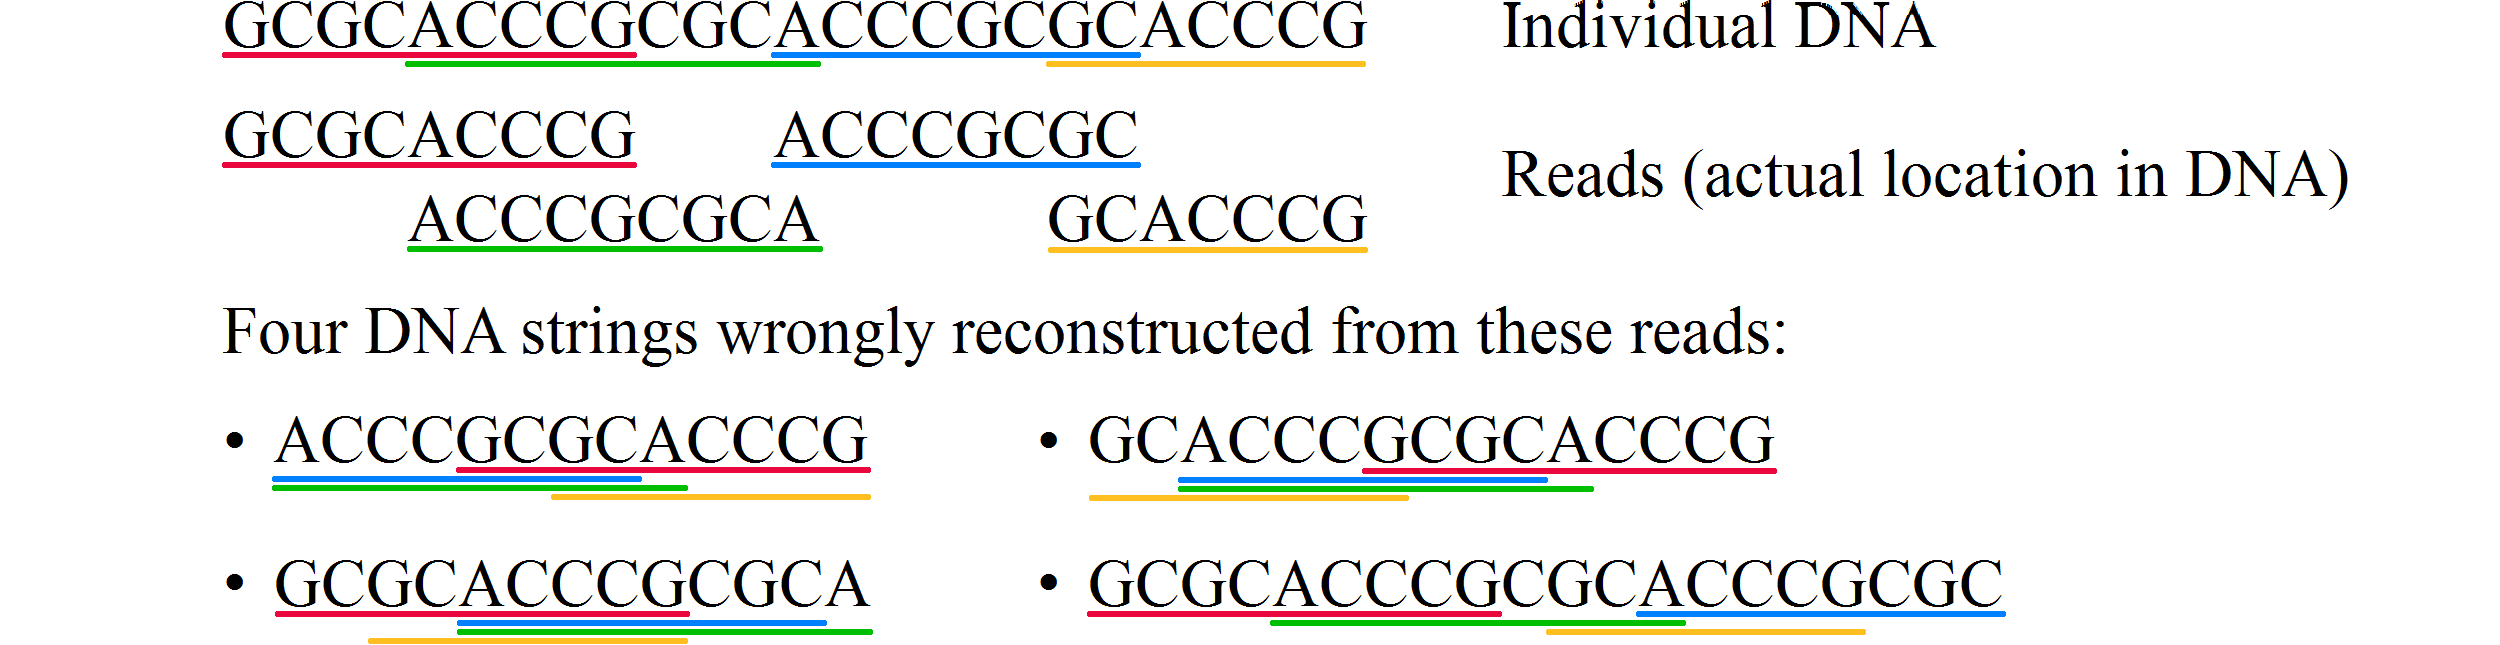
\includegraphics[width=\textwidth]{evo_intro_assembly_wo_reference.png}
\caption[Assembling an individual's DNA from small reads without a reference]{Problems with assembling an individual's DNA from small reads without a reference. Four possible reconstructions of the individual's DNA are shown, which all correspond to the observed reads, but are different from the actual DNA of the individual.} \label{fig:evo_intro_assembly_wo_reference}
\end{figure}
One purpose of the reference is therefore to guide the construction of the individual DNA in a meaningful way.
% TODO :: add picture and some text, saying: E.g. if we have the reads BLA then we could assemble them like BLA BLA,
% but with a reference we get BLAAABBEL...

Another purpose of using a genomic reference becomes clear 
in the case of diagnosing a disease in a patient. 
It is usually not very helpful to build the patient's full individual DNA, as the plain DNA string without 
annotations would not give us any information. 
% TODO :: citation needed
Instead, we are interested only in the variations from the norm, 
as these might be known to be associated with a specific disease. 
By aligning the reads to the reference, the software pipeline can keep track 
of the encountered differences and in the end give out a list of differences between the individual and the reference. 
An example for the process leading to such a list of differences 
can be seen in figure~\ref{fig:evo_intro_general_variation_calling_process}. 
\begin{figure}[!htb]
\centering
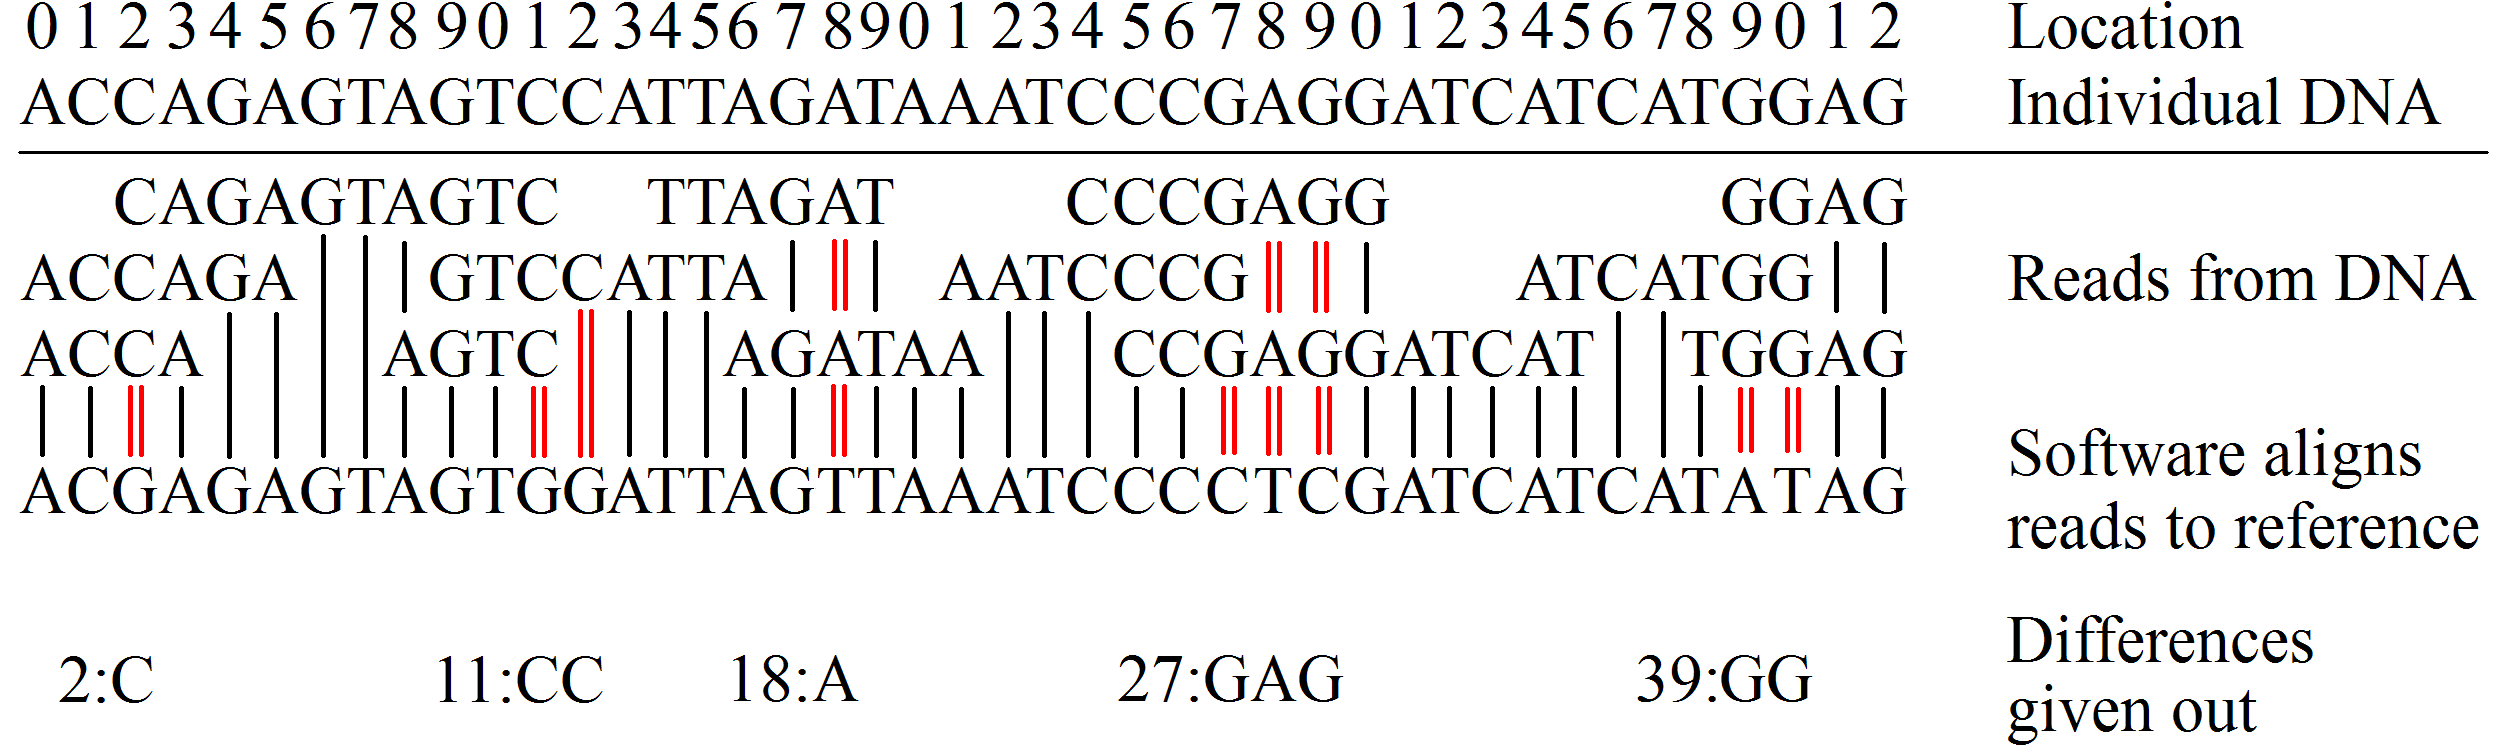
\includegraphics[width=\textwidth]{evo_intro_general_variation_calling_process.png}
\caption[General variation calling process]{General process for generating a list of variations between the individual DNA and the reference.} \label{fig:evo_intro_general_variation_calling_process}
\end{figure}
The alternative would be to construct the entire individual genome, and upon being done with this enormous task to 
compare the genome with a reference to find all the differences. This comparison however would be a sizeable 
and difficult alignment problem in its own right, so that it is more sensible to align the reads directly to the reference 
and give out the differences that were found in that way.

The reference therefore serves both as a blueprint while aligning the reads, 
as well as an anchor point to which variations within the individual string can be marked.

\section{The Reference Graph}

Traditionally, the reference is a compressed genomic string. 
In its simplest form it can be thought of as a plain text containing only the letters 
A, C, G and T. \\
It is rather straightforward to use such a reference string. 
Each location within the string can clearly be identified by its position---that is, 
its distance from the start. \\
Also, there are very simple file formats available to work with 
such references. One of these is the FASTA format, which includes the genomic 
strings together with lines for free text comments and with line breaks which 
make it easier to display the file in even low level text editors.
% TODO :: citation or link needed for FASTA (also, is it called FATA

The simplicity of reference strings however also has disadvantages. 
Most importantly, when aligning reads to a reference string, we can only align 
the reads to the average human genome, instead of aligning them to all known 
variations of the human genome at once. 
Not taking the known variations into account can lead to worse alignment results 
than would be possible otherwise, as the average genomic string may simply not 
include the particular mutations that have occurred for both the individual 
whose DNA is supposed to be read out as well as for another individual whose 
variations from the reference are known.

This is not just a theoretical consideration. 
Researchers now have access to annotated population variations, which augment the reference sequence string. 
These annotated variations can be found in databases of common variations, such as the publicly available  
dbSNP\footnote{\,\,\,\url{http://www.ncbi.nlm.nih.gov/SNP/}} 
and SNPedia\footnote{\,\,\,\url{http://www.snpedia.com/}}. 
Even the latest release of the Human Reference Genome, 
which is designated GRCh38
\footnote{\,\,\,\url{http://www.ncbi.nlm.nih.gov/projects/genome/assembly/grc/human/}}, 
contains alternative haplotypes for some complex regions, 
which are essentially known variations of the rigid reference string. \\
Considering that many alternative references are available and a lot of short variations are known, 
it becomes clear that the human genome should be thought of as a collection of individual genomes 
rather than a single rigid reference genome.

Algorithmically, this corresponds to viewing the reference as a graph rather than a linear genome. 
On this graph, each variation can be represented as a branch which points to the available alternatives. 
Thereby each personal genome is represented by a path through this variation graph, 
as can be seen in figure~\ref{fig:evo_intro_three_ref_seq_align}. \\
% TODO :: in the following picture, also add a graph interpretation underneath what I am seeing
%         (I want to see nodes and edges!)
\begin{figure}[!htb]
\centering
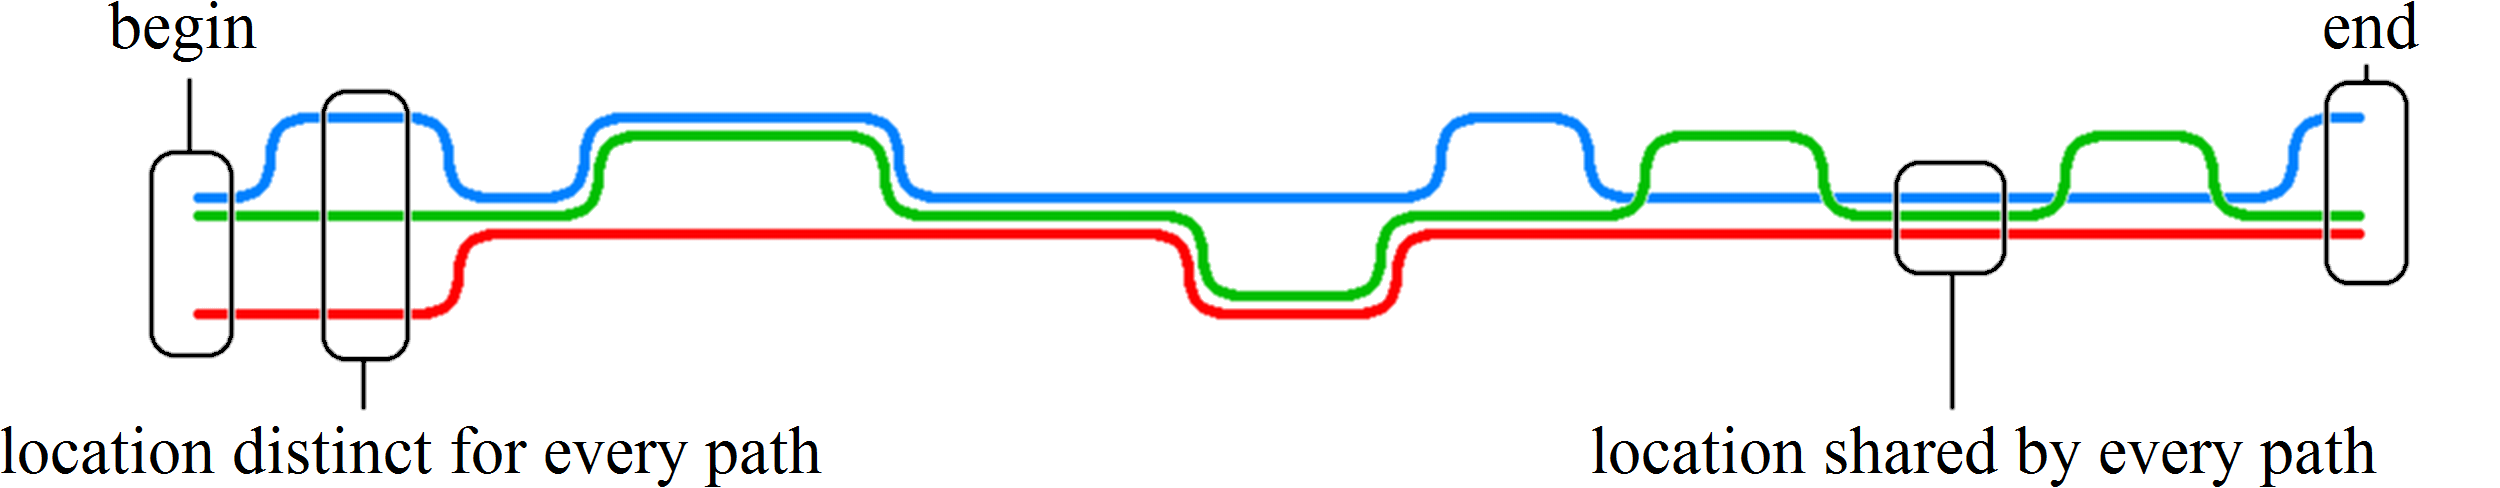
\includegraphics[width=\textwidth]{evo_intro_three_ref_seq_align.png}
\caption[Schematic visualization of three paths through a variation graph]{Schematic visualization of three paths through a variation graph, each representing an individual's genome.} \label{fig:evo_intro_three_ref_seq_align}
\end{figure}
This approach simplifies the identification of common variants, as a variant caller can 
ideally just note which path has been taken through the reference graph instead of having to 
explicitly state which differences have been found in which positions. \\
Using a reference graph also makes it possible to pick up combinations of variants 
which would currently be lost in the alignment step. 
Especially the calling of indels, which are usually harder to find and identify than edits, 
can benefit from having local access to several alternative references which contain 
already known variants \citep{Albers2010}.

Another advantage of using a reference graph presents itself when the continuous use of 
references over time is considered. 
When a new version of the human reference genome is published, 
it can take several years for research projects to adapt it, 
as existing pre-processed, aligned and annotated files all have to be updated \citep{RedditSwitchTo38}. \\
If instead a reference graph was underlying all alignments, it would be conceivable 
to update parts of that reference graph without changing the overall indexing of the entire structure, 
making it possible to seamlessly work with different versions of the entire structure. 
A possible way for a graph implementation to support this behaviour is by using a designated main 
reference that is unlikely to change often as the main indexing authority and by adding on top of it 
variations based on other references which can be changed out without changing the overall index.

Unfortunately, to fully implement a reference graph rather than a linear reference 
it is necessary to make drastic changes to all of the existing tools in the analysis pipeline. 
Such changes include the handling of new file formats which are capable of containing graph data, 
as well as changing the internal algorithmic logic of these tools to work on graphs.

\section{Thesis Motivation}

The focus of this thesis is therefore on the creation of an overview of the existing 
approaches that can be used for the implementation of genomic graphs, 
as well as on the exploration of new ways of working with genomic graphs, 
such as merging compressed graphs implicitly or explicitly. \\
The goal hereby is not mainly to create a new read alignment tool that uses 
a reference graph, but rather to create and implement new algorithms that can 
be used in conjunction with such graphs in the future.

Both the newly created algorithms as well as already established ones 
for the conversion of graphs between different internal formats 
will be implemented in such a way that their inner workings 
are directly observable. This simplifies the future usage of these algorithms 
within the scope of various parts of the analysis pipeline.

\chapter{Background}
% was ANDERE Menschen bisher so getan haben
%
% ====================================================================================================================================
%                                                                                                                           BACKGROUND
% ====================================================================================================================================

Nowadays there are many approaches for aligning short reads to a reference string, 
and even some work into the alignment of reads to a reference graph has already been 
undertaken.

\section{Burrows--Wheeler Transform Without Graphs}

The core problem of read alignment to a reference string is simply that a 
lot of data needs to be worked on, as both the reference itself is very big 
and the amount of reads is enormous. \\
This actually leads to two distinct problems, the first being that the 
memory requirements for storing any of the required data are huge, 
and the second being that the time that is spend aligning reads for 
even just a single individual is quite long.

To counteract the first problem, the data that is worked on is usually compressed, 
which means mostly that the string reference is being compressed in a certain way. 
A method that has been applied very often is the utilization of the 
Burrows--Wheeler Transform \citep{Burrows1994}, which 
in its original form consists of reordering a 
repetitive text with few runs into a text of the same length that contains more runs 
and can therefore be easily compressed by run-length encoding. 
A simple example of this behaviour can be seen in table~\ref{table:evo_background_bwt_run_enc}. 
\begin{table}[htb]
\centering
\caption[Run-length encoding comparison between a repetitive string and its BWT]{Run-length encoding comparison between a highly repetitive string and its BWT. In this example, the run-length encoding of the string itself does not reduce the size, while the run-length encoding of the BWT reduces the size by 29\%.}
   \begin{tabularx}{\textwidth}{ | X | X | }
   \hline
   AGCAGCAGCCTTCTTAGCCTT & \textbf{Original string} \\
   AGCAGCAG\,2C\,2TC\,2\,TAG\,2C\,2T & \textbf{Original string run-length encoded} \\
   \hline
   TCTCGGGGCTCAAAATTTCCC & \textbf{BWT} \\
   TCTC\,4\,GCTC\,4A\,3\,T\,3C & \textbf{BWT run-length encoded} \\
   \hline
   \end{tabularx}
\label{table:evo_background_bwt_run_enc}
\end{table}
As the transformed text contains all the information necessary to recreate the 
original text, it is not necessary to store the original text at all. \\
Many current alignment tools such as BWA-MEM \citep{Li2013} and Bowtie \citep{Langmead2009} use 
the BWT to compress the reference 
and even work on the reference in this compressed form directly, without having 
to recreate the original text in its entirety in memory.

As memory has gotten cheaper over time and machines have become more 
well-equipped, memory consumption nowadays is not as much of a concern 
as it once was, when just fitting the reference into memory 
took a lot of ingenuity. \\
% TODO :: citation needed
However, the memory utilization of alignment tools is still important, 
as further reductions in the overall amount of memory necessary would 
mean that the alignment could be done using smaller and therefore cheaper 
machines, which would open up more real-world applications for sequence analysis 
for which its price currently is still too high.
Also, a focus on how the available memory is used could lead to new alignment 
tools that make more efficient use of the special memory that is more readily available 
for the processor, such as using the L1, L2 and L3 cache rather than sending a lot of 
requests to the slower general RAM. \\
Therefore, research into methods reducing the memory requirements of alignment tools 
is still ongoing.
% TODO :: citation needed? maybe?

\section{The Role of Graphs in Read Alignment}

Initial use of graphs in read alignment was restricted to representing 
the outcome of the alignment phase, in particular the fully assembled DNA \citep{Myers2005}.

Short reads usually do not make it possible to fully infer the actual structure of the genome that is read out, 
as different possible structures could have lead to the same reads, especially when considering that 
there are many errors within the reads that need to be accounted for. \\
Therefore, often the reads are aligned to a reference and the best fitting position is simply 
assumed to be the real origin of the read. However, as the decision to choose one position over 
another can be quite arbitrary, graphs can be used as read alignment output which indicate how the reads 
are linked together. The true individual DNA that was read out is then one possible path through the graph, 
while other possible paths through the graph exist that are merely artefacts of the sequencing process. \\
As such a graph can be quite difficult to work with, not many alignment tools are producing these 
structures. Instead, the default is usually to just choose the best fitting position and 
create a read out DNA string. This string will most likely also contain some sequencing artefacts, 
but will be vastly easier to work with in later steps.

Graphs are currently also starting to be used as a way to reduce the size of several read out human 
genomes \citep{Li2014}. \\
The idea stems from the fact that companies or institutions that read out the DNA of several individuals 
and want to store them can run in problems with the immense file size when storing or transmitting the reads and their 
aligned locations. Instead, the original read data could be discarded and only the alignment result could be saved and shared---that 
however would mean that the original data cannot later on be re-interpreted by better algorithms, and can in general 
not be used any more. \\
Using a graph in this case can allow several agreeing reads to be combined into long sequences of unambiguous data, 
while the locations at which uncertainties exist could still be encoded with all the possible alternatives as 
different paths through the graph. Therefore, all complicated read data behaviour is contained in the resulting 
graph, but the size is still vastly reduced when compared to using all reference strings of the population.

\section{Burrows--Wheeler Transform for Graphs}

Graphs have not only been used to indicate the results of the read alignment. 
The alignment of short reads to a reference graph rather than to a linear reference has 
also been proposed several times.

A necessary prerequisite for aligning reads to a reference graph is 
being able to actually create such a graph in the first place. \\
One of these ways is to take several similar genomic strings and create a graph based 
on them, such that each of the input strings is a path through the resulting graph. 
\citet{Lee2002} proposed a method to create such a graph from input strings, 
independent of the order in which these strings 
are added to the emerging graph.

Storing several very similar references at the same time in a way that not only minimizes 
the storage space, but also enables efficient pattern searches directly on the 
stored data was proposed by \citet{Makinen2010}. \\
The aim of these techniques is to 
minimize both the overhead in storage space and the needed time to perform typical work 
on the references, such as aligning reads to them.

This group of authors continued working with scenarios in which 
several references are merged into a graph, with reads being directly 
aligned to the graph rather than to each reference on its own \citep{Siren2014}. \\
The alignment of reads against the data structure incorporating several references 
is done in a way that is inspired by the Burrows--Wheeler Transform. \\

In particular, to be able to use the Burrows--Wheeler Transform for read alignment, 
a data structure called the suffix array \citep{Puglisi2007} is commonly used, which contains 
information about the locations within the reference. 
Using the suffix array makes it easier to work on the BWT in its compressed form, 
rather than having to reconstruct the original string from it to perform work. 
That is, the BWT together with its suffix array forms a self-index, 
which is a data structure that contains compressed data and makes it possible 
to work on that data directly in its compressed form \citep{Navarro2007}. \\
As indexing a graph based on several references is not as straightforward as 
indexing a single string, which provides an inherent indexing mechanism by 
simply stating the position within the string, the regular suffix array cannot 
be used in the case of encoding a graph rather than a string. \\
However, the plain suffix array is often not used in a practical sense 
without any changes anyway. Instead, it is often compressed in some way or another. 
The reason for that is the immense size of the regular suffix array. 
A common compression technique is to leave out many of the suffix array's parts 
and instead compute them dynamically 
when they are being used rather than storing the entire array in memory. 

When using a reference graph for read alignment with the BWT, it is therefore common 
already to use a structure that simply behaves similar to the suffix array. 
Such a suffix-array-like data structure can also be constructed for graph references.

In particular, efficient support of the following operations is necessary for such a data structure \citep{Siren2014}: \\
Given a pattern, the range within the data structure 
that corresponds to all suffixes of the reference graph that are prefixed with that pattern needs to be found. 
This essentially provides a functionality for finding arbitrary texts, and is used when aligning reads to 
the reference, as that is basically a search for the read itself or similar patterns within the reference. \\
Given a location within the data structure, the corresponding location within the 
reference needs to be located. \\
Finally, given a location within the reference, the actual text at that position 
needs to be extracted.

The main idea is therefore to create a structure capable of fulfilling these requirements, 
as the remainder of the alignment step is then very similar to the alignment against a reference string.

\section{Alignment Without an Actual Graph}

To avoid the complications arising when working with 
a complete graph made from several references, other methods have been proposed 
to achieve similar results without explicitly constructing a reference graph.

One of these is the alignment tool BWBBLE which 
was created by \citet{Huang2013}. \\
It works on the core assumption that most differences in between two references 
are snips, which can be encoded with a specific extended alphabet. 
Then, a modification to the Burrows--Wheeler Transform is made to 
be able to work with a single string reference containing this extended alphabet. \\
BWBBLE also supports insertions and deletions which means that it does support 
more graph-like behaviour, but the core functionality of it is aimed at the extended string reference.

In addition, there have been efforts to more efficiently create the BWT 
of several strings rather than just concatenating them into a single one. 
These can help in understanding the challenges of building the BWT of several references \citep{Holt2014}.

\section{Using Hashes to Encode a Graph}

The hashing approach focuses also on a certain way of pre-processing the references 
to create a certain structure that the reads can then be aligned against. \\
To use this approach, a specific length $ k $ is given, up to which we keep track of 
sequences in the reference graph.

In the pre-processing step, among all the possible references one main reference is chosen. 
Then a hash table based on the references is created which 
assigns each $ k $-mer the positions at which it can be found. 
Such a position is not as straightforward as a 
plain integer that gives the index within a string, as the data can lie on branches 
off the main reference string. \\
This is solved by using an integer together with minor extra information. 
The integer points towards a data block, which can be a part of the main 
reference or a branch of any of the other references that differs from the 
main sequence. The extra information then points towards the location within the block.

In particular, aligning reads to several references at once 
in this way has been proposed by \citet{Schneeberger2009}. \\
In this case, the references are taken together to form a graph 
rather than being used as separate reference strings. 
For this to be achieved, all references are pre-processed in a special way, with one being taken as the 
main reference and the other references being stored as changes to this main reference. 
The pre-processing step results in a data structure that uses $ k $-mers as hashes pointing 
to the specific location at which these $ k $-mers can be found. Reads can therefore be aligned 
by finding parts of them in the hash table, looking up the locations that are associated with 
them, and checking if the entire read can be aligned to that location. \\
The location here is not just an integer pointing to a character within a string, 
as it would be for a single reference, but actually 
a pointer to the particular reference and the location within it. 
To make this indexing possible, the references are split into blocks that 
can quickly be addressed with an integer and locations within those blocks.

When the reads are aligned against the data structure, the output of the alignment step 
can be generated in two ways---either with each read being aligned to the particular reference 
that it agrees with most, or with each read being aligned in the same way but with the 
alignment afterwards being rewritten as if the read was aligned to the main reference. \\
This second option makes it possible to use this approach even as part of an already existing pipeline 
built for a reference string, not a reference graph, if losing some of the benefits of 
the graph alignment is acceptable. However, to fully utilize all the graph information, 
the rest of the pipeline has to be adapted as well.

\section{Extending the Burrows---Wheeler Transform}

Efforts involving changes to and generalizations of the Burrows--Wheeler Transform 
are also aided by the development of the XBW, which is a 
method of compressing trees similar to how the BWT is used to compress sequential data \citep{Ferragina2009}. \\
Each node in the tree has a label that is one character long. 
These labels are stored in the XBW together with a special bit vector, 
which keeps track of whether a given node is a leaf node or not. 
That is, if a node has a successor, then this bit vector takes the value 0, as that node is not the last node 
of its branch. If a node does not have a successor, then the bit vector takes the value 1 for that node. \\

\citet{Siren2014} extended the XBW even further, by introducing a second bit vector that enables nodes 
to have multiple predecessors as well as multiple successors. Therefore, this extended XBW can not only 
store trees, but instead can keep track of general finite graphs. 

\chapter{Methods}
% Lösungsansatz / VON UNS vorgeschlagene Methoden
%
% ====================================================================================================================================
%                                                                                                                              METHODS
% ====================================================================================================================================

To be able to understand the different existing approaches for working with 
reference graphs and genomic graphs in general, I have re-implemented several 
of these approaches myself. These implementations have been done in the programming 
language Python and resulted in several scripts that can be steered 
by a graphical main program written in Delphi. \\
I have then focused on creating the Graph Merging Library GML, which is a 
collection of algorithms written in JavaScript that make it possible to 
work with reference graphs in various ways. JavaScript is not a particularly fast 
language in itself, due to many inbuilt functionalities which are helpful for programming 
in it but slow it down compared to other languages such as C/C++ \citep{Taivalsaari2008}. 
The aim of this library is therefore not to directly provide a means to actually do 
real-world calculations using the entire human genome as reference graph, 
but instead it is focused on showing how different algorithms work, 
and in general to provide a test bed for working with genomic graphs. \\
Nevertheless, porting these algorithms to a faster programming language 
and using them in a production environment should of course be possible.

\section{Data Formats}
%
% ~~~~~~~~~~~~~~~~~~~~~~~~~~~~~~~~~~~~~~~~~~~~~~~~~~~~~~~~~~~~~~~~~~~~~~~~~~~~~~~~~~~~~~~~~~~~~~~~~~~~~~~~~~~~~~~~~~~~~~~~~~~~~~~~~~~~
%                                                                                                                METHODS: Data Formats
% ~~~~~~~~~~~~~~~~~~~~~~~~~~~~~~~~~~~~~~~~~~~~~~~~~~~~~~~~~~~~~~~~~~~~~~~~~~~~~~~~~~~~~~~~~~~~~~~~~~~~~~~~~~~~~~~~~~~~~~~~~~~~~~~~~~~~

In the course of working on this thesis I used existing data 
formats for genomic graphs and designed a new data format as well, 
to be able to better understand the strengths and weaknesses of 
the different possible approaches for encoding graphs.

\subsection{FASTG Format}

There are many formats readily available for genomic data strings 
that can be used when only sequential data is considered. 
One of the most common formats for genomic strings is the FASTA format. 
% TODO :: citation necessary
Its simple structure means that it is human-readable 
and can easily be used by various programs.

However, the aim here is to find data formats that are capable of 
encoding genomic graphs rather than strings. 
Such a format is FASTG, which is 
a FASTA-like format designed to handle graph data \citep{specFASTG}. 
Even though encoding genomic graphs is possible in the FASTG format, 
I noticed that it has some severe drawbacks.

Files in the FASTG format are unnecessarily big, which is mostly caused 
by a lot of intentional whitespaces but also by the decision to repeat the 
default interpretation of each FASTG-specific command just before the command. 
In the following FASTG example, the underlined 
text is just repeated and therefore unnecessary information:

...GCA\underline{TATGTCCTCTCTCC}[1:alt\pipe TATGTCCTCTCTCC\pipe GTC]GG...

On the other hand, when eliminating most of the whitespaces to reduce the file size, 
FASTG files which are already rather difficult to understand quickly 
become more and more obscure, such that they are no longer easily human-readable. 
However, that very human-readability is one of the main advantages of FASTA, 
and without it not much of a reason is left for using this particular family 
of formats altogether.

The FASTG format also is not very flexible. This can be seen by the fact that 
it only allows for three layers of variation within the entirety of the data. \\
The first layer considers global variation that is implemented through a mechanism in which the 
FASTA comments define which sequences can lead to which others. \\
The second layer is about local variation that is implemented through FASTG-specific constructs 
directly in the genomic data. \\
The third layer represents highly localized variation (such as snips) that can be nested 
inside of other FASTG-specific constructs from the second layer. \\
As not all of the constructs can be nested inside of each other 
and as the comment-based global and construct-based local 
variation are completely different approaches, this format 
seems unnecessarily complex.

Finally, the FASTG format as defined in 2012 with 
its many specialized constructs seems to be excessive for 
the needs of the Python test pipeline implemented in the course of this thesis. \\
Trying to implement the entirety of FASTG would in fact 
also be complicated by the fact that the format is open to amendments, 
such that solely implementing the existing standard would not be enough 
to be able to correctly work with all FASTG files which may be encountered. 
Even the specific bubble notation used within many FASTG files 
% which looks similar to ...ACGT[C,T]TAGT... 
does not actually occur in the standard written in 2012 \citep{specGFA1,specFASTG}.

\subsection{Bubble Format}

For very short and simple human-readable graph data, 
often the bubble format is used. 
It is not supposed to be used for production environments and indeed 
is not complex enough to describe any but the most trivial kinds of graphs. 
However, I still decided to also have a look into this particular format, 
as implementing it in a software package is rather straightforward due to 
its simplicity, and as considering it might teach us valuable lessons 
about problems to avoid when designing actual graph formats to be used for real world data.

In the bubble format a genomic sequence is represented as a single continuous string. 
There are no comments within the format, 
and neither newline characters nor in fact any kinds of whitespaces. \\
Any sort of graph representation in STPU is based on bubbles, which can be extended as long as necessary, 
and can be nested. A bubble is started with a “(” character and ended 
with a “)” character. Alternatives within the bubbles are marked with “\pipe ” 
characters. 
A representation of a short and simple graph in bubble notation can be seen in figure~\ref{fig:evo_fig_STPUbubble_f}. \\
Insertions and deletions are represented as bubbles whose alternative route is empty. 
One such deletion can be seen in figure~\ref{fig:evo_fig_STPUinsertion_f}. \\
As remarked before, this format cannot be used to represent arbitrary graphs. 
An example for which it fails to provide a correct encoding can be seen in figure~\ref{fig:evo_fig_STPUcycle_f}. 
Nevertheless, the bubble format is sufficient for simple algorithmic tests.

% \begin{figure}[!htb]
% \centering
% 
\includegraphics[width=0.47\textwidth]{evo_fig_STPUbubble_f.png}
% \caption[Simple bubble in STPU format]{Simple bubble, represented in STPU as \textup{ACGT(AG\pipe CTT)ATTTC}.} \label{fig:STPUbubble}
% \end{figure}
% ACGTCTTATTTC|,4,AG,8    nicer: AG against C - CGTAGATTC|,4,C,7 (without $ and #)
\begin{figure}[!htb]
\centering
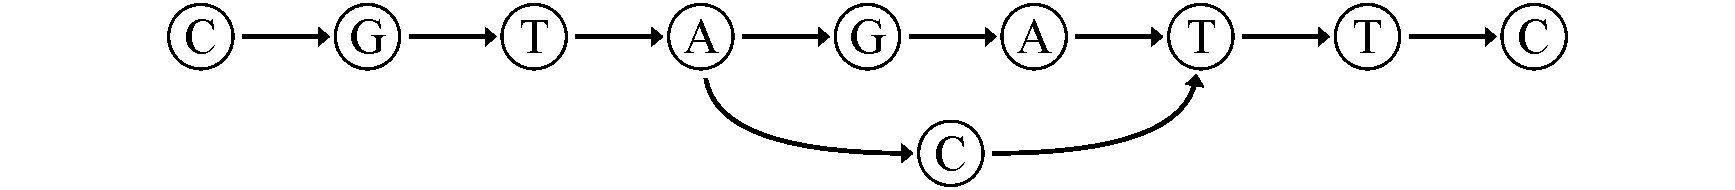
\includegraphics[width=\textwidth]{evo_fig_STPUbubble_f.pdf}
\caption[Simple bubble in bubble format]{Simple bubble, represented in bubble format as \textup{CGTA(GA\pipe C)TTC}.} \label{fig:evo_fig_STPUbubble_f}
\end{figure}
% \begin{figure}[!htb]
% \centering
% 
\includegraphics[width=0.47\textwidth]{evo_fig_STPUinsertion_f.png}
% \caption[Insertion in STPU format]{Insertion, represented in STPU as \textup{ACGT(AG\pipe )ATTTC}.} \label{fig:STPUinsertion}
% \end{figure}
% ACGTATTTC|,4,AG,5    nicer: deletion - CGTAGATTC|,4,,7 (without $ and #)
\begin{figure}[!htb]
\centering

\includegraphics[width=\textwidth]{evo_fig_STPUinsertion_f.pdf}
\caption[Deletion in bubble format]{Deletion, represented in bubble format as \textup{CGTA(GA\pipe )TTC}.} \label{fig:evo_fig_STPUinsertion_f}
\end{figure}
% \begin{figure}[!htb]
% \centering
% 
\includegraphics[width=0.47\textwidth]{evo_fig_STPUcycle_f.png}
% \caption[Cycle in STPU format]{Cycle, which cannot be fully represented in STPU, but can be approximated to any wanted length as \textup{ACGTAG(\pipe AG(\pipe AG(\pipe AG(\pipe ...))))ATTTC}.} \label{fig:STPUcycle}
% \end{figure}
% CGTAGATTC|,7,,4 (without $ and #)
\begin{figure}[!htb]
\centering

\includegraphics[width=\textwidth]{evo_fig_STPUcycle_f.pdf}
\caption[Cycle in bubble format]{Cycle, which cannot be fully represented in bubble format, but can be approximated to any wanted length as \textup{CGTAGAT(\pipe AGAT(\pipe AGAT(\pipe AGAT(\pipe ...))))TC}.} \label{fig:evo_fig_STPUcycle_f}
\end{figure}

\subsection{GFA Format}

The GFA or Graphical Fragment Assembly format 
has been proposed in 2014 \citep{specGFA1,specGFA2}. 
This young format has a lot of advantages over FASTG, mainly 
that it is a lot more flexible and can easier be read by programs, 
as not much emphasis is put on making it human-readable. Therefore, 
the focus can lie clearly on the readability for automated programs. \\
Unfortunately, GFA has several drawbacks as well.

A crucial problem is that GFA has only shortly been worked on, 
and no definitive standard has been published. \\
Although several people have responded quite favourably to the original blog post 
outlining the format, many have also come up with improvements and outright criticism, 
making it less likely that the format in its current state 
is already suited for implementation \citep{knightGFA1}. \\
The lack of a unified standard also means that it is not even clear which version of it 
to base an implementation on.

In the context of this thesis it is also important to consider another drawback. 
According to Heng Li, the author of the format, GFA only aims to be an assembly format \citep{specGFA3}.
% "GFA is not limited to an assembly format. It can represent arbitrary relationship between sequences and is thus suitable for a population graph format in theory. However, I would not take applications on population graphs, such as graph mapping, as a killer application of GFA. There are many open questions on population graphs. I cannot design a format for unsolved questions. GFA aims to be an assembly format only, at least for now."
This means that it can represent a graph based on one particular read assembly. \\
It has not, however, been designed to represent population graphs---which are exactly 
the reference graphs for which it would be helpful to have a useful format.

Finally, this format is very broad and allows for a lot of complicated 
graph behaviour, especially considering its elaborate CIGAR strings. 
This seems to introduce complexity that is, at least for now, 
unnecessary for the purposes of creating a simple 
implementation of a graph reference based alignment tool.

\subsection{GML Format}

While programming the Graph Merging Library, I decided to design a new format 
which could be used to encode genomic graphs. 
As both the FASTG and the GFA format seem to be rather extensive, 
the idea behind the GML format is to create a simpler way of encoding graph data. 
As can be seen with the success of FASTA files for sequential data, 
the simplicity of a data format is rather important, as it makes it more likely 
for future tools to be designed with inbuilt support for the format.

The aim of the GML format is also to not unnecessarily complicate the process of 
making existing tools of the analysis pipeline 
compatible with graph data. 
Therefore, the general structure of a GML-formatted file is similar to the general structure 
of a FASTA file, which is already widely used. \\
Namely, a GML file can contain comments and data, with different blocks of data being separated 
by comments. A comment in turn consists of the character “>” to indicate the start of a comment, 
the name of the following data block, followed by a space character and any free text that 
can be used as is deemed necessary when the file is created. 
If a GML file contains no comments at all, 
then all the rows are simply interpreted as one contiguous data block.

% TODO :: create general figure of GML file:
%

Within a data block, a genomic graph is encoded in two different parts. \\
The first part is referred to as the “main path.” 
This is simply the sequence of labels on any one path from the start node 
to the end node. The start and end nodes are labelled with a hashtag symbol and a dollarsign, respectively. 
These labels are not included in the main path within the file, as they are implicitly assumed 
to exist for any such graph. \\
The second part of a data block is optional. 
If the second part is given, then the first and second part of the data block are separated by a pipe character. 
This second part is an array of info blocks, separated from each other by semicolons. \\
Finally, each info block consists of exactly four parts which are separated from each other by commas.
\begin{itemize}
\item The first part is the identifier of the path, which can contain letters and underscores, 
as well as numbers in any position but the first. 
The identifier can also be left empty.
\item The second part is the origin of the path, 
containing the identifier of the path on which this one 
originates followed by a colon and the position within that path 
at which it originates. \\
The identifier of the main path is \texttt{mp}, but in the special case of the main path the 
identifier and the colon can be left out together, e.g. \texttt{mp:8} or just \texttt{8} for position eight 
on the main path, but \texttt{path9:8} for position eight on a path with the identifier \texttt{path9}.
Identifiers need to be defined before they can be used, that 
is, \texttt{AC|a,1,G,2;,a:0,C,3} is valid, while \texttt{AC|,a:0,C,3;a,1,G,2} is not valid. \\
The counting of the position starts at number zero for the first symbol. 
However, the main path implicitly contains the hash tag symbol and the dollar sign symbol. 
Therefore the hash tag symbol on the main path is \texttt{mp:0} and 
the first alphabetical character on the main path is \texttt{mp:1}, 
while the first alphabetical character on a path with the identifier \texttt{path9} is \texttt{path9:0}.
\item The third part is the content of the path, meaning the sequence of labels of nodes on the path. 
It can be empty if the path consists of just an edge from the origin to the target without containing any nodes.
\item The fourth part is the target of the path, 
specified according to the same format as the origin of the path in the second part of the info block.
\end{itemize}

% TODO :: create figure of GML file:
% e.g. GACG|p1,1,TGG,3;,p1:0,C,p1:2 or bubble notation G(A|T(G|C)G)CG
% mainpath|infoblock;infoblock;infoblock
% \                                    /
%             data block
%
% also have the actual graph representation of that with it on the figure =)

The GML format can encode any labelled graphs which start with a special hash tag node 
and end with a dollar sign node, as long as each node within the graph 
can be reached from the start and as long as the end can be reached from 
every node as well. These constraints are acceptable for practical use, 
as nodes that cannot be reached from the start would be ignored anyway, 
as well as leaf nodes that are not the end node. \\
Despite the potential to encode such complicated structures, it is reasonably 
simple and for very short graphs even human-readable. 
With increasing graph size the readability of a GML file without special software 
decreases though, as the info blocks containing alternative paths are quite not 
located close to where they are found within the main row, but are all concentrated at the end of the file.

\subsection{FFX Format}

In the process of creating GML, I finally designed one more data format for 
genomic graphs. The idea behind FFX, the Flat Fused XBW format, is to enable saving 
a flat XBW table directly, without having to convert it to some other format 
first. \\
As shown in subsection~\ref{sec:fusing_instead_of_merging}, 
it can be helpful to fuse several separate graphs together 
instead of merging them completely. Therefore, FFX is designed 
to specifically accommodate for these kinds of fused structures as well. 
It does not however impose these fused structures on the user, 
as non-fused graphs can simply be stored as single data blocks within 
an FFX file.

The basic structure of an FFX file is again inspired by FASTA, 
containing an optional starting comment which contains an identifier for 
the contents of the file and other text that can be used freely. 
The optional comment is then followed by one or several data blocks, 
with each data block being separated by comment lines. \\
However, if several data blocks are included within one FFX file, 
they are not seen as separate entities. Instead, the program working on 
the FFX file is supposed to handle them as fused flat XBW tables, 
with the end node of the first table leading into the start node of the 
second table, the end node of the second leading into the start node of the 
third, and so on. \\
As more complex formats are less likely to become 
used by the community at large as it would be harder to re-implement them 
in various situations, certain rules are imposed on these fused data structures. 
First of all, a data block is always fused to the one directly following 
within the file. 
Theoretically, it would be possible to create a set of rules for the comment 
lines to indicate that other relations should instead take place, such as the 
end node of the first table leading to the start node of the fourth and so on, 
but even though this would increase the flexibility of the format, it would only 
increase the difficulty of writing an implementation for it. 
Likewise, each data block is only allowed to contain exactly one hash tag node 
as start and exactly one dollar sign node as end. Therefore, the path from one 
data block to the next is always completely linear, and every path through the 
entire FFX file must use every edge between the data blocks exactly once. \\
At the first glance, this might seem like a rather limiting constraint. 
However, it should be noted that much more complex behaviour is very possible 
within each data block, which can encode a complex a graph as is necessary. 
Also, this is inspired by the actual needs for a huge graph reference, 
in which the overall structure is very linear and all perturbations are on a 
rather local scale.

In FFX, each data block consists of the BWT, the $ M $ and $ F $ bit vectors, 
and additional data which could be constructed on the fly from just the BWT, 
but which takes up a lot of time to be constructed while only take up a small 
amount of space, such that saving it explicitly within the file means that the 
lengthy process of computing it again and again does not need to be executed on 
every opening of the file.

% TODO :: make clearer HOW the BWT, M and F are encoded in a data block, and WHAT other data there is
% TODO :: add pictures of FFX files and the corresponding graphs (also a picture of two graphs being merged, leading to one data block, and two graphs being fused, leading to two data blocks)

\section{Python Scripts}
%
% ~~~~~~~~~~~~~~~~~~~~~~~~~~~~~~~~~~~~~~~~~~~~~~~~~~~~~~~~~~~~~~~~~~~~~~~~~~~~~~~~~~~~~~~~~~~~~~~~~~~~~~~~~~~~~~~~~~~~~~~~~~~~~~~~~~~~
%                                                                                                              METHODS: Python Scripts
% ~~~~~~~~~~~~~~~~~~~~~~~~~~~~~~~~~~~~~~~~~~~~~~~~~~~~~~~~~~~~~~~~~~~~~~~~~~~~~~~~~~~~~~~~~~~~~~~~~~~~~~~~~~~~~~~~~~~~~~~~~~~~~~~~~~~~

To get a better understanding of how a regular alignment 
pipeline works, I started by implementing one such pipeline on my own. 
The goal here was not to achieve a solution that could compete with 
the already commonly used alignment packages, but rather to have a 
simple test bed that I could then later on expand by slowly adding more 
and more diverse graph reference approaches.

\subsection{Chosen Programming Languages}

As speed was not of great concern, but ease of implementation was, 
I wrote this pipeline mostly in Python. The various Python scripts 
that correspond to individual steps in the alignment pipeline---mostly 
pre-processing the reference, aligning the reads to the reference, 
and assembling the aligned reads into the individual DNA---are however 
controlled by another program, which I wrote to have quick access to 
the alignment information and a simple overview of the current status 
at all times. A screenshot of this main control program can be seen figure~\ref{fig:MCC}. 
\begin{figure}[!htb]
\centering
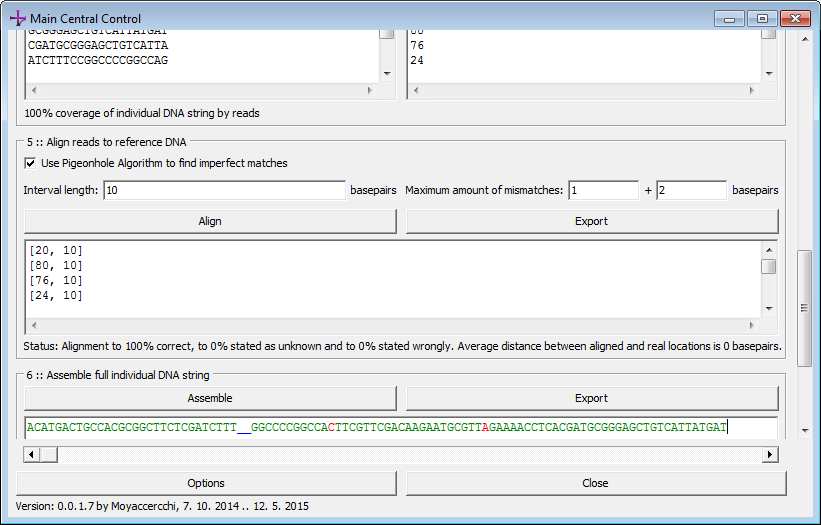
\includegraphics[width=0.95\textwidth]{evo_fig_MCC.png}
\caption[Graphical control program]{Screenshot of the graphical control program written in Delphi.} \label{fig:MCC}
\end{figure}
I have constructed this control program in Delphi, as implementing a GUI 
application in Windows is very simple with that language. \\
The program can automatically generate short artificial DNA reference strings, 
generate individual DNA with any amount of modifications---pure edits, 
but also insertions and deletions whose extent can be freely chosen. 
Then, reads of a chosen length stemming from an individual with that DNA 
can be automatically generated, optionally with a freely entered 
amount of random mismatches from the individual genome string. 
Further on, my Python programs for the read alignment and re-assembly of the original individual DNA 
as well as the variant calling 
based on the reference and the aligned reads are steered using that program. \\
All the steps from the creation of the random data to the end-result, 
the analysis of the quality of the alignment, can be accessed via this one interface.

\subsection{Quality Assessments}

Generating all of the data artificially means that it can easily be checked 
how well the entire tool chain performed, especially the read alignment phase, 
as the original positions from which the reads originated are known and can be compared 
to the positions that have been found. However, it is not necessary 
for this process to use random artificial data---instead, 
any sort of data can be supplied and used by it, 
in which case the analysis can simply result in showing how much 
of the reconstructed string actually matches the individual DNA that the reads were based upon, 
if that string is known. \\
If that original string is not even known, 
the string reconstruction can still occur, but the final analysis of the 
reconstruction quality is then limited. In that case, it mostly consists of analysing 
how well the aligned reads fit together during assembly, which can show problems that 
have occurred if many reads with contradicting information were aligned to similar positions. \\
To make that analysis, the Python script that is responsible for assembling the 
aligned reads into the final resulting genomic string considers for each of the $ n $ positions 
the information from all overlapping reads. If the reads all agree in a position $ k $, 
then the alignment quality $ q_k $ there is perfect or $ 100\% $. If some reads propose a certain 
character and some others indicate a different character, then the quality of 
the position is calculated as the amount of reads supporting the chosen character $ a_\textrm{s} $ 
divided by the total amount of reads $ a_\textrm{t} $ that contain information about that position.
\[ q_k = {\frac{ a_\textrm{s} }{ a_\textrm{t} }} \]

The overall assembly quality $ q $ is given as the sum of all individual character qualities, 
divided by the amount of characters.
\[ q = {\frac{ \sum\limits_{k=1}^n q_k }{ n }} = {\frac{ 1 }{ n }} \sum\limits_{k=1}^n {\frac{ a_\textrm{s} }{ a_\textrm{t} }} \]

An example of the assembly quality assessment can be seen in figure~\ref{fig:PYTHONqualityass}.

% Position $ i $ 0 1 2 3 4 5 6 7 8 9 10 11 12 13 14 15 16 17 18 19 20 21 22 23 24 25 26 27 28 29 30 31 32 33 34 35 36 37 38 39
% 
% Read 1 AAGGATATTGAAACTCCAATTTTCTCTAGA
% 
% Read 2 AAGGAAATTGAAACTCCATTTTTCTCTAGA
% 
% Read 3 AAGGATATAGAAACTCCATCTTTGTCTAGA
% 
% Read 4 ACGGAAATTGAAACTCCATCTTTCTCTAGA
% 
% Read 5 AACGATATTGAAACTCCATTTTTCTCTAGA
% 
% Assembled DNA AAGGATATTGAAACTCCATTTTTCTCTAGA
% 
% Quality $ q_i $ 1.0 0.8 0.8 1.0 1.0 0.6 1.0 1.0 0.8 1.0 1.0 1.0 1.0 1.0 1.0 1.0 1.0 1.0 0.8 ...

\begin{figure}[!htb]
\centering
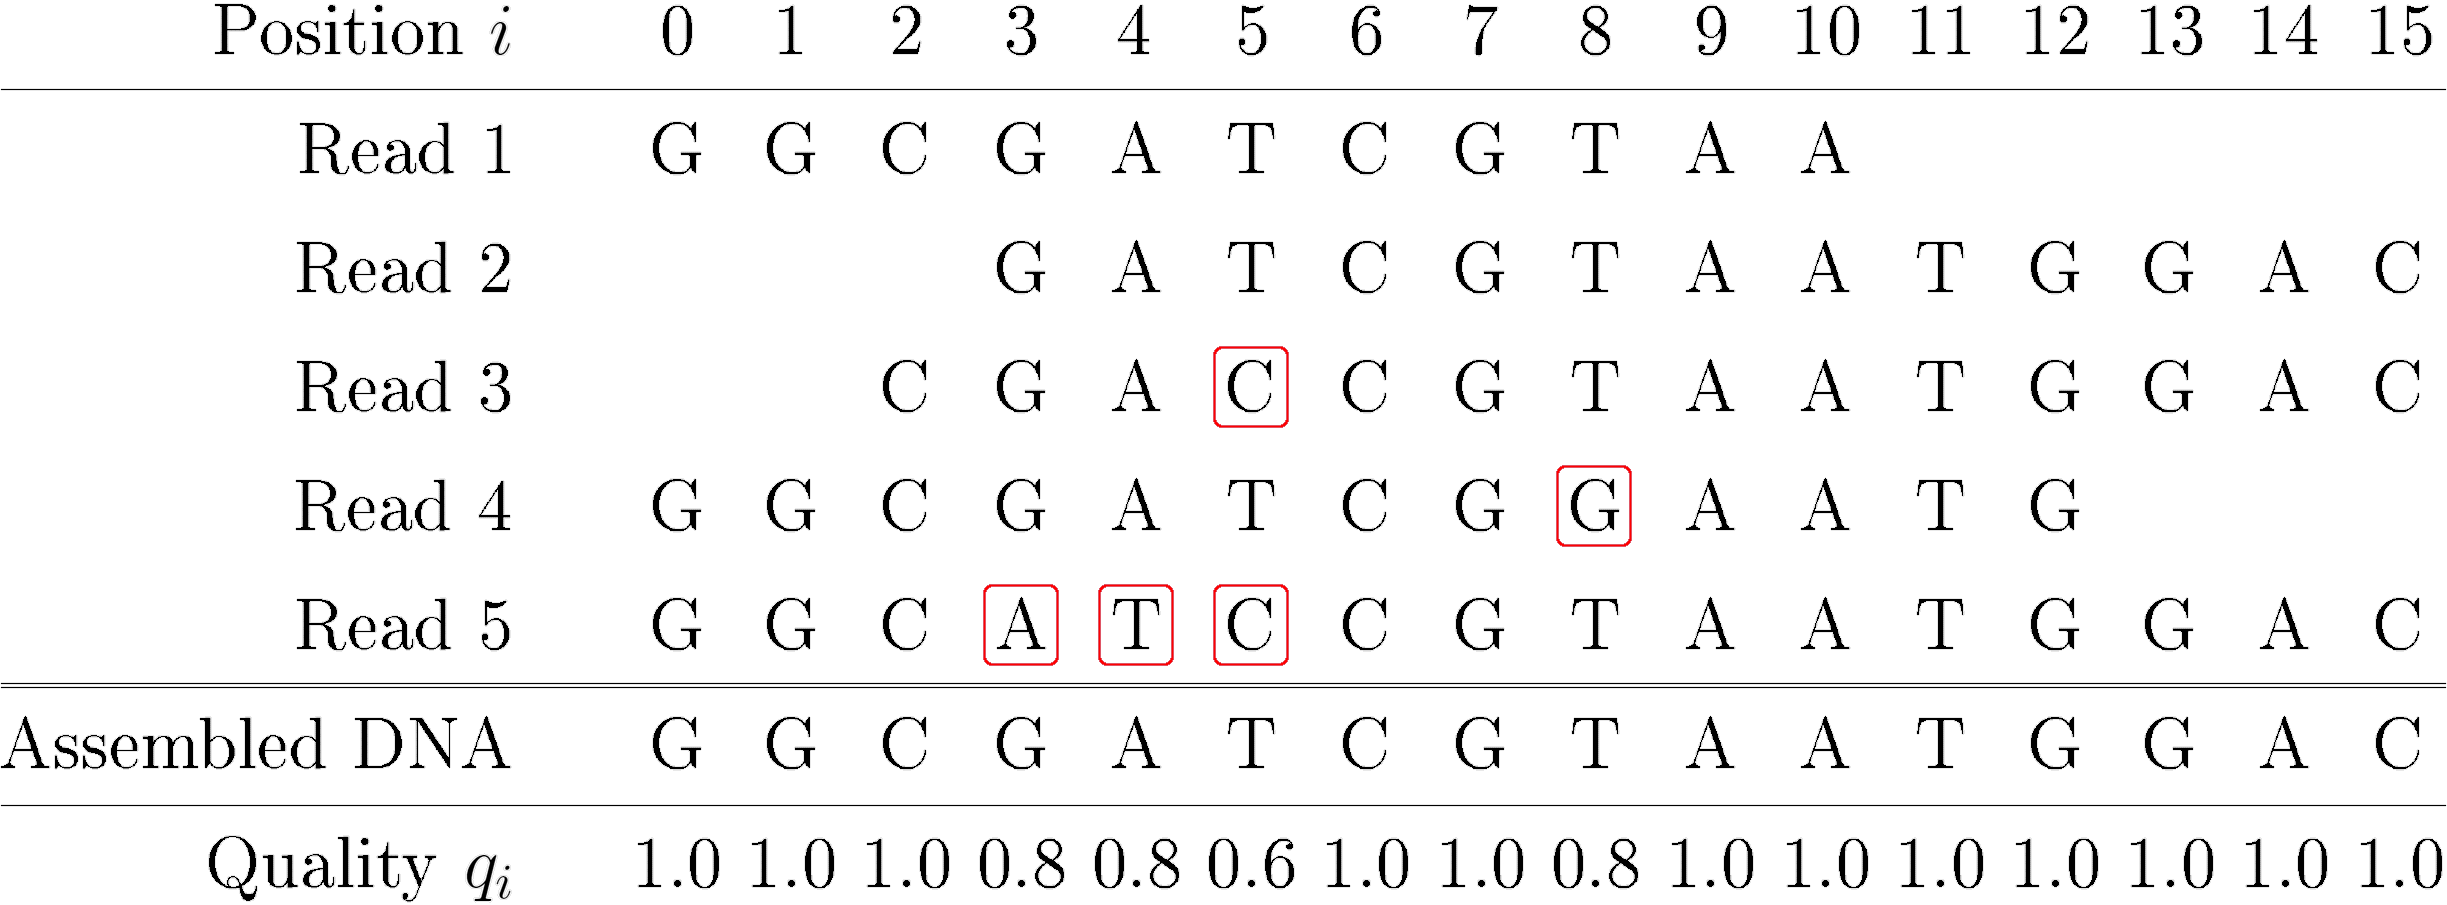
\includegraphics[width=0.95\textwidth]{evo_fig_PYTHONqualityass_f.png}
\caption[Assembly quality assessment]{Assembly quality assessment with five reads that span parts of the assembled DNA.} \label{fig:PYTHONqualityass}
\end{figure}

\subsection{Improving the Minimal Working Package}

The implementation of the core functionality of the 
assembly pipeline was rather straightforward. However, 
at that point the alignment script was built around the 
assumption of perfect, noise-less data---ideally with the 
individual DNA that is supposed to be read out being the same 
as the reference DNA that is given, or only being different 
in a few distinct locations where simple edits appeared. \\
Real-world datasets on the other hand are inherently noisy, 
and the differences between the reference and individual DNA strings 
are usually much more complex, including insertions, deletions, 
and even the displacement of entire blocks of characters.

Therefore, one of the first core improvements was to not only allow 
for a handful of edits but also handle insertions and deletions 
with the overall tool chain. That is, the alignment tool manages 
to align reads to the reference which contain insertions or deletions relative 
to that reference. In that case, not just the position of the read relative 
to the reference is returned, but also additional information about the location of the insertions and deletions 
needed for the read to fit to the reference. \\
The read assembly program uses that information to estimate the real location of insertions and deletions 
from the noisy results that the sum of all reported insertions and deletions represent and 
then assembles the original DNA using that information.

Another improvement was focused on the parameter $ d $ for the alignment script. 
The alignment is based on the pigeonhole principle, in which up to $ d $ mismatches 
between two strings that are supposed to be aligned to each other are accounted for by splitting one of the strings 
into $ d + 1 $ parts and aligning them individually. As there are at most $ d $ mismatches in 
every aligned location that we intend to find, 
at least one of the parts must be exactly contained in the other string at that location. 
We keep track of the locations at which at least one part is aligned perfectly, and then 
count for each of these candidate locations if an alignment of the entire string brings no more than 
$ d $ mismatches. \\
This process ensures that all locations in which the two strings are aligned with 
up to $ d $ mismatches are found. 
Despite that, there is a slight problem with this process: Ideally, $ d $ should be increased to be 
able to find even the most misshapen alignments, as real data is very noisy. 
But a higher $ d $ parameter means drastically more work that needs to be done, and a lot more runtime 
being spent.

To counteract this problem, and allow for more mismatches without having to increase the “expensive” (with 
regards to computing time) parameter $ d $, I introduced a new parameter $ k $ for the alignment script. 
As before, it is assured that all locations at which the read aligns to the reference with up to $ d $ 
mismatches are found by the script. However, with only a slight increase in runtime we are also given 
the chance to find locations with up to $ d + k $ mismatches as well. \\
This works by still splitting the read into $ d + 1 $ parts and aligning them individually, 
but then checking the candidate locations while allowing for $ d + k $ mismatches rather than just $ d $ 
mismatches. To see that this process does not in fact guarantee finding all 
locations at which the read aligns with $ d + k $ mismatches, it is enough to consider the 
case of $ k = 1 $ with one mismatch being contained in each of the $ d + 1 $ string parts. 
As in that case none of the parts match substrings of the other string, no alignment will be reported. \\
In real data however, mismatches usually 
cluster together rather than being spread out evenly, 
% TODO :: citation needed
such that the chance for finding alignment locations with 
up to $ d + k $ mismatches is good, while the additional cost is very small.

% TODO :: add a figure (or 9) to better explain the d+k business!
% [FIGFIGFIG] [F3]

\subsection{Simple Graphs}

After having improved my pipeline in the aforementioned ways, 
I started working on the focus of this thesis: Using a population graph reference 
rather than a string reference as basis for the read alignment.

To not have to tackle the entire problem immediately at once, 
I started by focusing on very simple graphs with highly specific requirements 
as to what kinds of structures they could and especially could not contain. 
These highly specific requirements meant that the implementation complexity 
was greatly reduced.

In fact, the first graph-based 
version of my pipeline only accepts graphs with non-nested snips that have 
two alternatives, each being of length 1. \\
This means that a reference such as AAGT(C\pipe T)C would be allowed, 
containing the snip (C\pipe T). However, (CT\pipe G(A\pipe G)) would not be 
allowed due to the non-nested requirement. Also (C\pipe A\pipe G) would 
not be allowed, due to the requirement of the snips having exactly two alternatives. 
And finally (CT\pipe GA) would not be allowed due to the requirement of each 
alternative path being of length exactly 1, neither allowing for empty paths nor 
for longer ones. \\
It is clear that these requirements are preventing all but a tiny subset of 
real-world problems from being worked on, but they are a good starting point for 
thinking about the general approach for the implementation of a graph-based 
reference.

To implement this reduced graph problem, several stages in the pipeline needed to 
be modified. First of all, the random generation of the reference string was 
set up to also generate the allowed snips.

A bit more complicated were the necessary changes for the pre-processing script. 
The script was amended to output not just the pre-processed 
reference, but also a graph-free reference string, which the later scripts 
could then use as simple integer-indexed reference sequence instead of the graph reference itself. 
This made it possible to 
re-use these scripts without changing them at all. \\
In particular, the reference AAGT(C\pipe T)C would be saved as AAGTCC, 
which is an ordinary reference string corresponding to the first path through 
the graph. Using this string for read alignment and assembly obviously works 
great if the individual DNA actually corresponds to the first path being 
taken through the population reference graph---that is, if the individual DNA 
at that position was AAGTCC. However, even if the individual DNA corresponded 
to the other alternative, which is AAGTTC, it would still be very likely for the 
alignment and assembly to work on this genomic sequence. Part of the reason for that is that 
a few mismatches are allowed for anyway to make up the inherent noise of any dataset. 
On top of that though not all stages are relying on this modified 
reference graph---in fact, the read alignment stage is mostly concerned with the 
pre-processed reference anyway, and only uses the given reference string to confirm 
potential alignment sites.

The second change to the pre-processing script concerned the general approach that the script 
should take while working through the reference. \\
For a string reference an iteration over the reference is enough to build up a pre-processed structure. 
In the first simple test implementation I actually let a Python script build up a hash table explicitly, 
by writing down every $ k $-mer within the reference, 
its origin from within the string 
and sorting the strings alphabetically. \\
The length $ k $ was here chosen to be exactly the same 
as the part length $ h $ used later on during the pigeonhole algorithm. 

% TODO :: add a figure about how regularly I am building up the thing
% [FIGFIGFIG] [F2]

With the inclusion of short, non-nested snips into the reference, this approach changed in several ways. \\
The pre-processed data structure was still built by iterating over the reference (which is simply read as a string in 
the STPU format). Just like before, the first $ h $ characters of each suffix are written out explicitly 
until a bubble is encountered---that is, until a “(” character is seen as the last character of the suffix that is written out. 
Once such a character is encountered, something different needs to happen. 
First of all, the length $ h $ over which each suffix is read needs to be expanded. 
However, it is necessary to still keep track of the original length $ h $, 
so instead $ h^{\prime} $ is introduced. 
It is set such that the read out part of the suffix actually spans $ h $ characters 
when accounting for taking different alternatives in the bubble. \\
This means that $ h^{\prime} $ starts out at the value of $ h $, but can change while 
iterating over the reference to account for different read window lengths. 
On the other hand, $ h $ stays invariable while iterating over the reference 
and describes the length of the prefix of the suffix that is written onto the list. \\
Also, instead of just plainly writing out the $ h^{\prime} $ first characters of the suffix, 
the different suffixes that arise from making the possible choices for the bubble are written out. 
So when we are looking at a suffix with the first $ h^{\prime} = 8 $ characters being ACG(C\pipe T), 
actually ACGC and ACGT are added to the output, both with the same origin location as suffix array entry. \\
The iteration then continues by advancing one letter. The bubble is now contained within the region of 
the suffix that is read out, and again all possible alternatives are written into the output. \\
The iteration in which the left-most character that we are reading out is the starting “(” character of 
the bubble is the last iteration before we return to using $ h $ instead of $ h^{\prime} $. 
Also, we are afterwards increasing the position by 4 to jump over the remainder of the bubble. 
This behaviour will be changed when considering longer bubbles, but is adequate for the very basic case 
that is considered here.

% TODO :: add a figure about how we are doing it now (with 1-long non-nested 2-snips)
% [FIGFIGFIG] [F1]
% base it on the longform comment in step 2, but do not use the verbatim environment -
% instead actually build it in paint etc. as usual!

One last remark should be made about the number that is used for indexing. 
When using a string reference that contains no graph aspects at all, we simply use one counter $ i $ 
to iterate over the reference and write out the current value of the counter. \\
However, using the graph reference we are basically losing positions in the reference to graph features 
which take up space in the original reference string, but do not contribute to the actual location within it. 
Therefore, a second counter $ i_{\textrm{absolute}} $ was included which keeps track of where in the 
equivalent string reference the current location is. \\
To illustrate this more clearly, consider the beginning of a reference that starts with ACACCAT(G\pipe T)AC. 
For the first 7 positions, $ i $ and $ i_{\textrm{absolute}} $ would contain the same value, so 
value 0 for “A”, 1 for “C”, 2 for the next “A” and so on. In position 7 (which is the eighth character, “(”,
as we are starting to count from 0), we still increase both of them together, as the 
contents of the bubble take up a space. However, for the next four positions---corresponding to the characters “G\pipe T)”---only 
$ i $ is increased (as the actual location in the graph input is increased), while $ i_{\textrm{absolute}} $ is 
not changed. Finally in position 12, at “A”, $ i $ has the value 12 while $ i_{\textrm{absolute}} $ has the 
value 8. \\
In general, $ i_{\textrm{absolute}} $ always corresponds to the current location 
in a reference that could be created from the actual graph by just choosing the first alternative. \\
In fact, this is precisely the new adjusted reference that is given out by this script, as explained before.

% TODO :: add a figure about exactly these i and i_absolute values, just to also SEE it; as seeing 
%         is much more helpful than explaining!
% [FIGFIGFIG]

\subsection{Further Considerations}

The problem stated earlier---allowing for non-nested snips with two alternatives, each of length one---was 
already very much reduced. And yet, two small problems that have not been mentioned so far 
can still arise, even in that very simple scenario.

% in the next paragraph we have:
% snips before the end of the first virtual read (so basically pre-processing for the pre-processing;
% in our script, this is done as a small while-loop just before the main loop)

The first of these two problems arises when snips are contained in the very beginning of the reference. 
As mentioned before, the horizon $ h $ which describes the length for which output string entries 
are made is expanded to $ h^{\prime} $ whenever the current window's rightmost position features the start of a snip. 
If a snip starts far enough in the beginning of the reference that its start lies to the left of the rightmost position of the 
very first window, then it would be ignored and the resulting output would not contain strings 
of the correct length.

% TODO :: show how the snip or bubble needs to lie, and what the leftmost rightmost middlemost position is ;)
% [FIGFIGFIG]

To counteract this problem, a small loop was added to the beginning of the pre-processing script, 
which iterates over all the characters to the left of the rightmost character of the first window 
and sets $ h^{\prime} $ to the correct value. Of course, as $ h^{\prime} $ is the length of 
the window over which the reference is read, a higher $ h^{\prime} $ means that the first window 
is longer, and therefore the loop needs to change the position at which it ends based on the $ h^{\prime} $ 
that is generated within it.

% in the next paragraph we have:
% two snips (or even more) within one virtual read

The other problem concerns the spacing between two snips within the graph. \\
If we only consider one snip at a time, then the solution thus far presented works. 
On the other hand, when several snips are contained in the reference, 
the distance between the snips relative to the original horizon $ h $ is important. 
Is that distance above $ h $, then again the presented solution works, as 
each snip is encountered individually. Is that distance smaller, 
then the snips are encountered within the same window. \\
In that case, first of all $ h^{\prime} $, which had been expanded to $ h + 4 $, 
needs to be expanded again. It is then 8 characters longer than the original horizon, with 4 characters 
for each snip. In fact for every new snip encountered $ h^{\prime} $ needs to be expanded by 4. \\
Also, the increased amount of possibilities need to be taken into account when the 
suffixes are added to the list. E.g. when looking at ACAT(G\pipe C)ATA, the strings 
ACATGATA and ACATCATA need to be added to list, but when looking at ACAT(G\pipe C)A(T\pipe A)A, 
the strings ACATGATA, ACATGAAA, ACATCATA and ACATCAAA need to be added. 
To achieve this, an implementation was used that started out with a set containing just the substring in question, 
and on each iteration replaced every string in the set with all the strings that 
are generated by replacing the first bubble within the string with every path through it. 
Only when none of the strings in the set contained any bubbles at all anymore were 
they all individually added to the pre-processed data structure.

% TODO :: a figure, I NEED a figure here! strings with strings with paths with what? ;)
% (maybe use the aforementioned string ACAT(G\pipe C)A(T\pipe A)A in the figure, or not...)
% [FIGFIGFIG]

\subsection{Straightforward Generalizations}

The graphs that have been considered so far were drastically reduced in complexity to allow for the simplest possible 
implementation. 
Generalizing the previous approach all the way to general graphs is not very straightforward, mostly because the 
system of counting with $ i_{\textrm{absolute}} $ relative to an adjusted reference string relies on the fact that 
all alternative routes through the graph have the same length, which is an unreasonable assumption for real-world data. \\
% TODO :: maybe a citation for the real world data having different path lengths through bubbles?
% (basically anything that points towards insertions / deletions on an individual-specific level would already be helpful here...)
However, there are a few generalizations that can easily be implemented immediately.

First of all, there is no particular reason to enforce that a bubble should only contain two alternatives, 
such as (A\pipe T). Instead, allowing snips with any number of alternatives, such as (A\pipe T\pipe C) and 
even just (A) to support slightly malformed input is much more reasonable. \\
To do so, it must be noted that the extra length of a snip as opposed to a regular letter was 
so far exactly 4 characters. Now however a snip can span as little as two extra letters in the example of (A), 
or also a lot more than just 4 characters. To make the previous implementation work with such snips, 
the code simply needs to look out for the next “)” character after the opening of the snip, and 
keep track of the distance between the two. \\
Also, the code that chooses all possible alternatives through the graph and adds each of them to the suffix array 
needs to now allow for more than 
just two alternatives, which again is straightforward to implement.

% in the paragraph that follows, we have:
% each path with a length higher than just 1 (this actually makes it necessary to not jump out of 
% the snip directly, so we really should write a fair bit about it!)

Another quickly implemented generalization centres around the length of the paths 
within the snips. By looking at bubbles instead which contain longer alternative paths, 
more general problems can be tackled. \\
This means that instead of limiting the program to recognize a snip like (A\pipe G), 
a bubble like (AT\pipe GC) can also be recognized. 
Even before implementing this explicitly, 
two snips could have been combined to (A\pipe G)(T\pipe C) to achieve a similar outcome to that bubble. 
However, it would not have been exactly the same, as the bubble only allows for AT and GC, while the 
approach with two snips allows for any combination of the letters in the first snip 
and the letters in the last, meaning AT, AC, GT and GC being allowed.

It here needs to be noted that even when we allow bubbles with path lengths 
above 1, we still require all paths through a bubble to have equal length. 
Therefore, (ACC\pipe TGT) would be allowed with the new script, 
but (ACC\pipe T) would still not be allowed, as one path is three characters long 
while the other is only one character long. \\
The reason for holding up this requirement is that again the entire idea 
of working with an absolute reference indexing via the variable $ i_{\textrm{absolute}} $ and 
a re-written reference string is based on all possible paths through all graph blocks 
having the same length. This approach alone simply cannot work in a case in which 
several paths have different lengths, as the indexing of the reference would not 
be able to match the indexing of the pre-processed suffix array. 
For these cases, a different solution is necessary.

To actually let the pre-processing script handle bubbles with several characters 
in each alternative, it is necessary to base the change to $ h^{\prime} $ not 
only on the amount of alternative paths, but also on their length. 
This can simply be achieved by searching for the next occurrence 
of the “)” character and adding the distance between the opening and closing 
of the bubble to $ h^{\prime} $, as was already introduced before anyway 
to allow for more than one alternative. \\
Also, the part of the script that builds up the entries to the pre-processed table 
themselves needs to be changed to account for taking several characters at a time, 
which again is rather simple to achieve by taking all characters until the next “\pipe ” character. \\
The most challenging change to script the actually stemmed from the fact that now 
it is not sufficient any longer to jump over the entire bubble when the opening bracket 
has been encountered in the left-most position of the window, as we in that 
case lose the suffixes starting within the bubble. Instead, we have to advance the 
window inside of the bubble and only jump to its end by increasing $ i_{\textrm{absolute}} $ and 
decreasing $ h^{\prime} $ once an amount of characters has been encountered equal 
to the length of an alternative route. Again, all alternatives are assumed to have 
equal length, so this can simply be implemented by keeping to iterate until the first “\pipe ” character 
is encountered. \\
Finally, allowing bubbles with several characters in each alternative also 
makes it necessary to add an explicit limitation on the length of string that 
is added to the pre-processed list. 
Basically, as $ i_{\textrm{absolute}} $ is increased by the total length of the 
bubble, it is increased $ n * (l - 1) $ characters further than technically 
necessary where $ n $ denotes the amount of alternatives in the bubble, and $ l $ denotes 
the length of every alternative itself. We can see that for snips, in which $ l $ is equal to one as 
each alternative only consists of one character, the increase is zero and does not need to be 
taken into account. However, when $ l $ increases, it does need to be taken into account, which 
can be done by simply adding the first $ h $ characters of the suffix that is found to 
the pre-processed list. This is equivalent to what was being done before, but then 
there was no need to explicitly call for the first $ h $ characters, as they were given 
by the algorithm automatically. \\
Having $ i_{\textrm{absolute}} $ at a value higher than technically necessary and simply 
taking only the first $ h $ characters of the output could at the first glance seem wasteful and 
impractical; however, this practice allows to iterate over the last window positions before 
jumping over the rest of the bubble without having to move the actual window, 
as all positions are then calculated automatically, which actually simplifies the 
algorithm. Otherwise, the it would need to keep track of being inside of a bubble but 
being past its starting point while iterating over the reference.

% TODO :: make a figure for what came before (especially in the second-last sub-paragraph)
% [FIGFIGFIG]

% TODO :: maybe indicate in the previous paragraph's last sub-paragraph a bit more that this is ONE WAY
% of doing it, that we chose now for ease of implementation, but not necessarily the BEST way of doing it ;)
% (and that's fine, as long as we are aware of it and maybe even build the other one too and time it...)

Lastly, both of these generalizations make it necessary to track how much $ h^{\prime} $ has 
been changed to make it possible to undo these changes when leaving the snip or bubble. 
Before, as only snips with two alternatives were allowed, $ h^{\prime} $ was always increased 
by 4 and decreased by 4 when leaving the bubble, increasing $ i_{\textrm{absolute}} $ by 4 as well. \\
Now, we keep track of the increases that have happened in a list. We append new increases to its end, 
and take the old increases off from its beginning when they are needed 
to keep track of the different amounts. So we might append the increases 6, 4 and 12 to the list 
for the bubbles (AC\pipe TG), (A\pipe T) and (AGT\pipe CCC\pipe GTA), and when leaving 
the first bubble get the value 6 from the list which was appended at first, later on the value 4 and 
as last one the value 12. We are therefore using a first-in, first-out queue.

% TODO :: add a figure about the improved bubble-jumping stuff for alternatives of length above 1 each
% [FIGFIGFIG] [F4]

Altogether, this allows already for more complicated graphs, 
but still two key problems remain, namely the implementation of nested bubbles 
as well as the implementation of bubbles with alternative routes that have different lengths. 
These are especially important as they are used to minimize the size of the file that is worked on 
and to describe insertions and deletions, 
which with the system presented so far could not be represented at all. 
Furthermore, tackling general graphs is even more complicated but also even more 
helpful in real-world applications.

\subsection{Nested Graphs}

The stated problem can be further generalized by not just allowing flat bubbles, 
but by actually accepting nested bubbles within the reference. 
So instead of just accepting A(GT\pipe GC\pipe CT)G, the reference A(G(T\pipe C)\pipe CT)G could 
be accepted, which describes the same three strings: AGTG, AGCG and ACTG.

Any nested bubbles can theoretically be flattened to non-nested bubbles. 
Using them however means that long repetitions of nearly identical alternative paths in 
bubbles can be avoided, reducing the required file size and potentially improving the 
memory requirements and the execution speed. \\
As any nested bubble can just be flattened, two ways for working with nested bubbles can be identified:

\begin{enumerate}
\item Flatten out the reference before pre-processing it, 
which would mean to transform A(G(T\pipe C)\pipe CT)G into A(GT\pipe GC\pipe CT)G before 
applying anything else
\item Directly pre-process the reference containing nested bubbles, 
which is more complicated to achieve but does not make it necessary to 
introduce a new step before the actual pre-processing
\end{enumerate}

I have implemented the second of these possibilities, for which again 
a few changes needed to be made to the Python script that pre-processes the reference.

% TODO :: also implement the first of these possibilities maybe? And make comparisons
% (which should hopefully show that the second way is better for file size (simple), memory (öööhhh) and speed (ayayay))

First of all, the script that creates an adjusted, flattened reference 
needs to work for nested bubbles as well, again choosing the first alternative within any bubble. \\
So GA(GC(T\pipe C)A\pipe CAGG)T(G\pipe A)C needs to become GAGCTATGC. \\
To better keep track of this activity, I encapsulated it into a new function 
within the script called \texttt{flattenreference}. \\
In previous versions of the script this worked by finding the first bubble within a given string, 
and then combining the text before the bubble with the first alternative within the bubble and 
the text after the bubble, repeating this until no more bubbles are left. \\
In particular, in GA(GCTA\pipe CAGG)T(G\pipe A)C we would first concatenate GA, GCTA and T(G\pipe A)C 
to find GAGCTAT(G\pipe A)C, see that there is another bubble, and then concatenate 
GAGCTAT, G and C to finally find GAGCTATGC.

This approach would have worked with nested bubbles too, but it would have been unnecessarily complicated 
to keep track of the nestedness with it. Instead, the new approach is a bit different. \\
Considering the example GA(GC(T\pipe C\pipe A)A\pipe CAGG)T(G\pipe A)C, 
this string is split on the first “(” character into two parts, GA and GC(T\pipe C\pipe A)A\pipe CAGG)T(G\pipe A)C. 
This is done recursively until no more “(” characters are left and the parts are GA, GC, T\pipe C\pipe A)A\pipe CAGG)T 
and G\pipe A)C.\\
Now from each of these parts, the text between the first \pipe and the first “)” character is taken out (including both 
of these characters) iteratively until no more \pipe or “)” characters are left.\\
This gives the parts GA, GC, TAT and GC, which are in a final step concatenated to finally get 
GAGCTATGC.

% TODO :: add a figure about the previous paragraph?
% later me: yepp, do that! =)
% [FIGFIGFIG]

The second change to the script needed to happen in the actual pre-processing phase. 
This phase is mainly based upon three numbers which are constantly reassigned. 
They represent the beginning of a bubble, its middle length (meaning the length of one of its alternatives), 
and its end position. \\
Finding the beginning of the bubble did not change, as finding the first “(” character is still sufficient here. \\
However, to find the middle length and end position, two new functions have been introduced which do more 
work than was necessary before.

In \texttt{getbubblemidlen}, the middle length is found by iterating over the inside of the bubble 
one character at a time, and keeping a list of levels which keeps track of the alternative being the first 
on each level. \\
To make this more clear, assume the string GT(CT\pipe TA)G\pipe CAA(A\pipe G)A representing 
the inside of a bubble. In the beginning we start out at a nestedness of level 0, and we are in the first alternative 
path, so the list contains one element which is \texttt{true}. As all elements of the list are \texttt{true}, 
we add the first two characters to the count and get a preliminary count of 2. \\
The next character is “(”, so we add an element to the list which also contains the value \texttt{true}. 
For the next two characters, C and T, all elements of the list are \texttt{true} so each of them is 
added to the count, reaching 4. \\
The following character is “\pipe ”, so the last element of the list is set to \texttt{false}. 
During the following characters, T and A, nothing is added to the count as not all elements of the list are \texttt{true}. \\
Upon encountering “)”, the last element is taken off the list, such that it now contains only one element, 
that one still being \texttt{true}. Therefore, the next character is counted, to reach a count of 5. \\
When the central “\pipe ” is encountered, the only element on the list is set to \texttt{false}, 
so that all other characters are no longer counted, as the list will always contain this element. \\
The final count is therefore 5, which represents the length of the bubble if the first alternative is always 
chosen. Due to the assumption that all paths have equal lengths, it at the same also represents the 
length of every other path.

% TODO :: add a figure about the previous paragraph?
% [FIGFIGFIG]

A different approach for finding the middle length would have been to call the function \texttt{flattenreference} 
on the bubble itself and to count the length of the resulting string.

The other new function is \texttt{getbubbleend}, which cannot simple find the position of the first “)” character, 
as that one may belong to a bubbled nested inside the one that is currently considered. 
It instead finds the position of the “)” character that closes the first “(” character. \\
To do so, an iteration is done which in each step jumps to the next “(” or “)” character. 
If the character is “(”, a variable that keeps track of the depth is increased by one, 
while otherwise it is decreased by one. When the depth, which started out at one after finding 
the first “(” character, reaches zero, the correct position has been found.

% TODO :: add a figure about the previous paragraph?
% [FIGFIGFIG]

Overall, these changes mean that now arbitrary combinations and nesting schemes of bubbles can 
be accepted within the reference string, as long as the one main assumption still holds true, 
which is that all paths through the bubbles need to lead to the same length within the adjusted reference.

\subsection{Truly Arbitrary Graphs}

Overcoming the last hurdle means to make it possible to accept graphs that contain paths of different 
lengths along parallel edges, such as the simple bubble contained in GT(A\pipe CT)GT. 
As this can both be read as GTAGT and GTCTGT, it is not clear how the indexing after 
this fragment should proceed, as it could have taken either 5 letters or 6 letters.

The simplest solution to circumvent this problem seems to be to simply rely on the ability of the 
alignment program to recognize indels. In that way, the reference could count 5 letters for 
GTAGT, while actually GTCTGT is read out, with one extra insertion.

% TODO :: maybe move the following three paragraphs to a more suitable place?

When enabling this within my own script I noticed a problem about the general indel handling 
that had not been addressed before, as it had never really come into focus until then: When 
there is an indel, it can be hard to figure out whether an insertion or a deletion has taken place, 
especially if it occurs close to the ends of the read. \\
Assuming a read like GCAG and a reference like GCATG, the read could be aligned to the first position 
within the reference, and the last character of the read could be seen as edit (with a “T” in the reference becoming a “G”), 
could be seen as insertion (with a “G” being inserted after the “A” in the reference) or it could be 
seen as deletion (with the “T” in the reference being deleted.) \\
In practice, an indel being mistakenly interpreted as edit operation was not very problematic, 
as then only this one read was shifted, but the other reads at that position overpowered the one 
that was wrongfully shifted. However, it often occurred that insertions were wrongfully interpreted as 
deletions, and vice versa.

To counteract this, I first noticed that it makes no sense to assume an insertion and a deletion at the 
exact same location. If most reads report that there is either an insertion or a deletion, then 
using both within the program leads to no offset change and therefore all the indicators pointing to 
indels would be ignored. \\
Therefore, if a location contained both insertions and deletions, they were both seen as the class 
that contained more evidence. So if there were 10 reads at a certain location, with 7 of them 
pointing towards an insertion at that location, 2 of them pointing towards a deletion and 
1 pointing towards an edit operation, then these would be seen as 9 insertion supporting reads, 
as the deletions would be changed to insertions. This was also applied the other way around.

The reason why this makes sense is that some reads contain the indel close to their middle. 
In that case, the read should have enough data on both sides to accurately determine whether 
this is an insertion or a deletion. \\
% TODO :: add a figure about this
% [FIGFIGFIG]
On the other hand, the wrong classification of insertion or deletion usually stems from reads 
for which the indel lies at the very beginning or end, so that context information is only available 
on one side of it. \\
These are just as likely to report insertions as deletions, while the reads that contain the 
indels in the middle are more likely to report the correct classification. 
Therefore, taking the class that has more evidence going for it means giving emphasis to 
the reads that contain the indels in their middle, which are more trustworthy.

With these changes, the pipeline was finally able to use arbitrary graphs.

\section{Graph Merging Library}
%
% ~~~~~~~~~~~~~~~~~~~~~~~~~~~~~~~~~~~~~~~~~~~~~~~~~~~~~~~~~~~~~~~~~~~~~~~~~~~~~~~~~~~~~~~~~~~~~~~~~~~~~~~~~~~~~~~~~~~~~~~~~~~~~~~~~~~~
%                                                                                                       METHODS: Graph Merging Library
% ~~~~~~~~~~~~~~~~~~~~~~~~~~~~~~~~~~~~~~~~~~~~~~~~~~~~~~~~~~~~~~~~~~~~~~~~~~~~~~~~~~~~~~~~~~~~~~~~~~~~~~~~~~~~~~~~~~~~~~~~~~~~~~~~~~~~

After gathering experience on how to implement a pipeline used for aligning reads to a reference in general, 
I decided to create the Graph Merging Library. 
\begin{figure}[!htb]
\centering
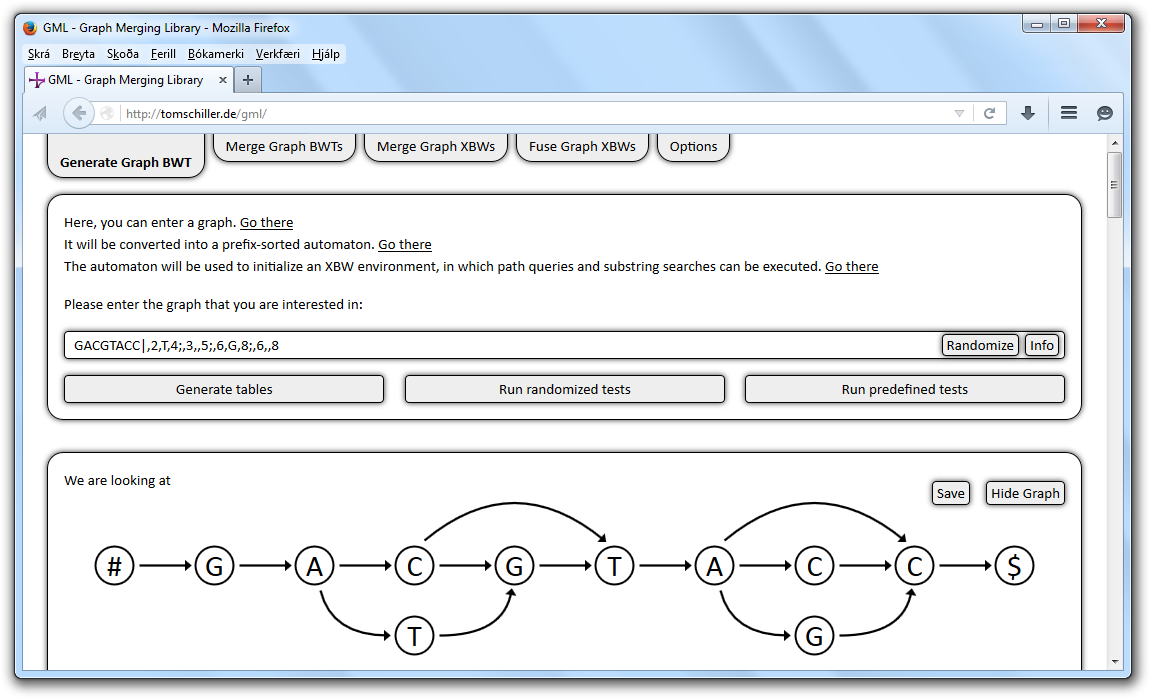
\includegraphics[width=0.95\textwidth]{evo_gml_3.png}
\caption[GUI of the Graph Merging Library]{Graphical User Interface of the Graph Merging Library} \label{fig:evo_gml_3}
\end{figure}
This is a software library written in JavaScript, with a graphical user interface written in HTML and CSS, 
that can be used to more explicitly understand how various algorithms for working with genomic graphs work. 
A screenshot of user interface can be seen in figure~\ref{fig:evo_gml_3}. \\
In particular, GML includes different methods for merging and fusing genomic graphs, 
which may be helpful to other future projects.

\subsection{Generating a Genomic Graph}

To use a genomic graph in the Graph Merging Library, 
a GML file can be opened which contains the desired graph. 
In the graphical user interface, not only can such a GML file be opened, 
but a valid GML data block can also be entered directly within an input 
field to simplify getting started with the software. 
If such a file has been opened, then some work still needs to be undertaken 
to convert the opened graph into the extended XBW format. \\
The extended XBW format requires for each graph for start with a node labelled with a 
hash tag sign and to end with a node labelled with a dollar sign. 
When opening a GML file, these extra nodes are therefore created first, and the 
main row as specified in the GML file is added between them as one possible way 
of traversing the graph from the hash tag node to the dollar sign node. 
Then the info blocks are iterated over, and their contents are added as edges and nodes.
% TODO :: add algorithm: The entire process is illustrated in algorithm~\ref{alg:...}.

\subsection{Visualizing the Graph}

After opening the graph, it can be helpful to show it to the user for 
quick and easy visual inspection. 
I therefore included a small visualization function within the Graph Merging Library, 
which is capable of displaying simple graphs nicely. 
Algorithm~\ref{alg:visualize} shows how this function works in general. 
\begin{algorithm}
\caption[Visualize a graph]{Visualizes a graph by first displaying one path from 
the starting node to the end node, referred to as main row, 
and then adding alternative paths around the established core.}
\label{alg:visualize}
\begin{algorithmic}[1]
\State $ \textrm{current\_node} \gets \textrm{graph}[0] $
\Comment{Display main row}
\State \textbf{draw} current\_node
\State $ \textrm{more\_nodes} \gets [ \, ] $
\While {current\_node.label \textbf{is not} \$}
	\State \textbf{append} current\_node \textbf{to} more\_nodes
	\State $ \textrm{current\_node} \gets \textrm{current\_node.successors}[0] $
	\State \textbf{draw} current\_node
\EndWhile
\State \phantom{emptyline}
\ForAll {more\_nodes \textbf{as} path \$}
\Comment{Display other paths}
	\State $ \textrm{current\_node} \gets \textrm{path} $
	\If {current\_node has not been drawn}
		\State $ \textrm{node} \gets \textrm{current\_node} $
		\State $ \textrm{path} \gets [ \, ] $
		\While {node has not been drawn}
			\State \textbf{append} node \textbf{to} path
			\State $ \textrm{node} \gets \textrm{node.successors}[0] $
			\If {node has not been in more\_nodes before}
				\State \textbf{append} node \textbf{to} more\_nodes
			\EndIf
		\EndWhile
		\State \textbf{draw} nodes \textbf{in} path together
	\EndIf
	\ForAll {current\_node.predecessors \textbf{as} predecessor}
		\State \textbf{draw} edge \textbf{from} predecessor \textbf{to} current\_node
	\EndFor
\EndFor
\end{algorithmic}
\end{algorithm}
Having a closer look at line 1 of the algorithm, 
it can be seen that it constructs the main row 
by starting in the first node, which is assumed to 
be labelled with the hash tag symbol. 
In line 6 of the algorithm it can then be seen 
that to construct the main row starting with this node, 
the algorithm always jumps into the first of the successors of the current node. \\
Therefore, before a graph can be passed to the visualization function, 
it needs to be ensured that its hash tag node is stored in the very first position 
and that the node labelled with the dollar sign can be reached by always travelling 
along the first of the successors. 
A separate function called \texttt{makeAutomatonPretty} is used to ensure that this is always the case, 
by traversing all possible paths and picking one path which leads to the dollar sign node. 
In the options it can be chosen whether this function 
should find one of the shortest paths, which is faster, or one of the longest paths, 
which leads to a better visualization. 
When it is instructed to find one of the longest paths, it will however still ignore 
paths including loops, as it might otherwise be trapped in the loop indefinitely, 
trying to find yet longer paths. 
An example for how this choice affects 
the visualized graph can be seen in figure~\ref{fig:evo_fig_visualize_short_vs_long}.  
% merge GACGT|,2,T,4;,3,,5 vs. ACCT|,1,,4;,1,,3, once with normal settings, once with forcing shortest path
\begin{figure}[!htb]
\centering
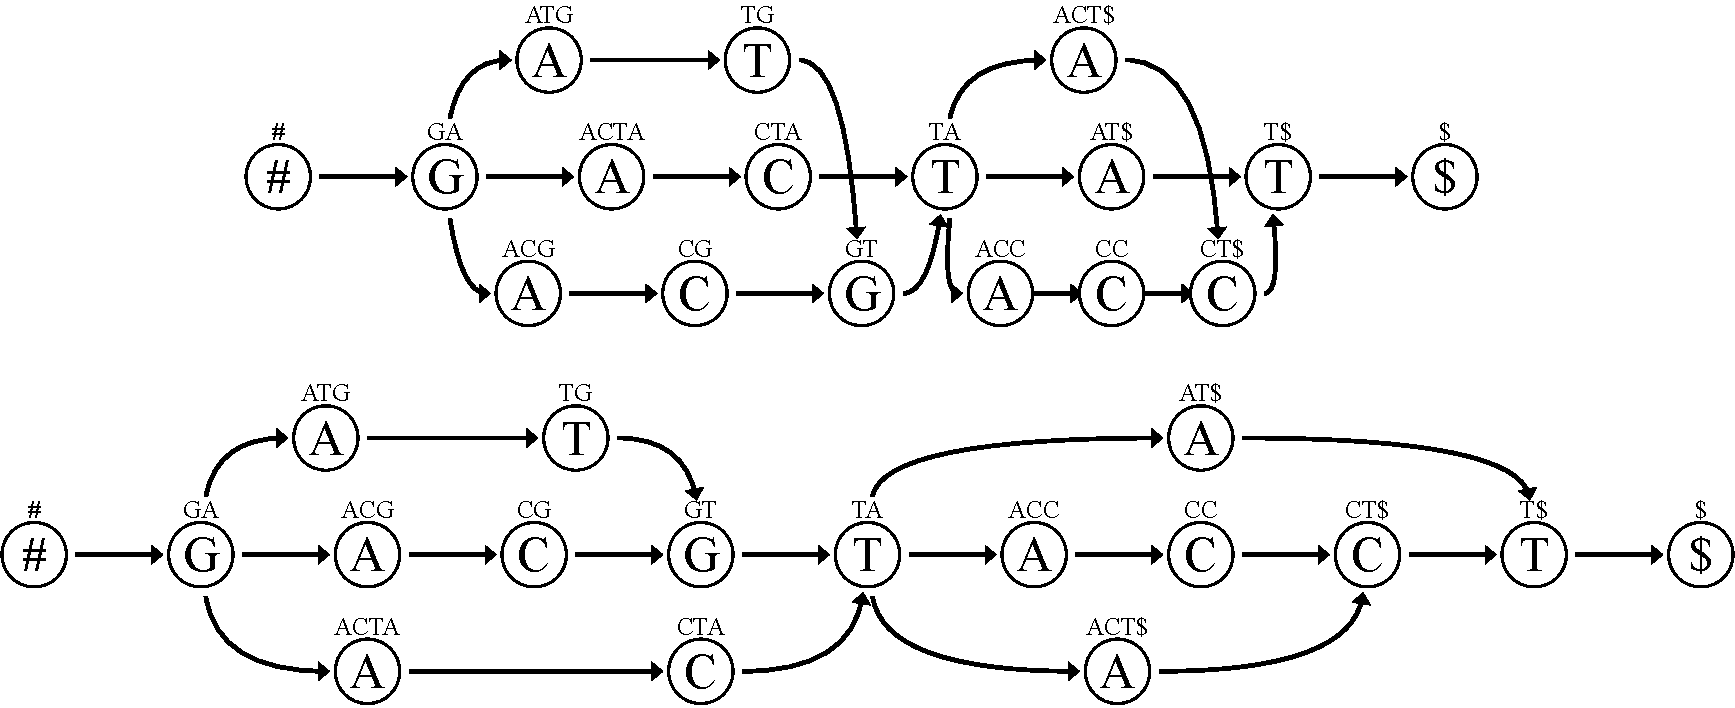
\includegraphics[width=\textwidth]{evo_fig_visualize_short_vs_long.pdf}
\caption[Visualizations of graph with shortest and longest main rows]{Two visualizations of the same graph. The visualization on the top uses the shortest possible path as main row, while the visualization on the bottom uses the longest possible path.} \label{fig:evo_fig_visualize_short_vs_long}
\end{figure}
The graph nodes are then adjusted in such a way that following the first successor of each 
node upon starting at the hash tag node leads directly to the dollar sign node. \\
It is also notable how exactly the iteration over the nodes works out. 
In line 10 we iterate over all nodes that have been added to more\_nodes, 
an array which keeps track of nodes which we have not fully worked on yet. 
This means that we may have already drawn the node, but we have not yet 
drawn all the incoming edges, and we may possibly not even have drawn the node itself. 
The loop in line 15 then iterates over all the first successors of that node, 
and adds them to an array called path, until a node is encountered that has already been drawn. 
Finally, in line 22, the entire path is drawn together. \\
Algorithmically it would be much more straightforward to simply iterate over all nodes 
and draw them when we encounter them, but in that case we would not have a good idea about 
where it might make sense to draw them. The approach of iterating over nodes 
that have not been worked on and nesting into this an iteration of the successors of that node 
allows us to instead draw entire parts of paths at once, so that we have a good idea 
where exactly to put the nodes on the display when drawing them, as they can simply 
be arranged next to each other.

\subsection{Ensuring the Graph is Reverse Deterministic}

Having displayed the graph, we now continue working on it to ultimately be able 
to work with it in the extended XBW format.

For any node within the graph, we can construct a prefix, 
which is the sequence of its own label concatenated with the labels of the nodes which are 
traversed when exiting that node. 
% TODO :: insert image about prefixes and how they are generated 
% (even through strands that are split apart, but have identical labels)
The extended XBW compression scheme for graphs as proposed by \citet{Siren2014} relies 
on the possibility of ordering all nodes of a graph alphabetically, based on their prefixes. 
After opening a file format that can contain arbitrary graphs, 
it is therefore first of all necessary to ensure the graph is reverse deterministic, 
as otherwise at least two nodes could not be unambiguously sorted against each other. 
File formats which can contain graphs which are not reverse deterministic include 
FASTG, GFA, GML and the bubble format, while the FFX format guarantees that 
the stored data is reverse deterministic as its entire encoding paradigm 
otherwise would not work. \\
% TODO :: insert figure in which we can see a non-reverse deterministic graph and the prefixes being the same.
To understand why a graph not being reverse deterministic would lead to 
at least two nodes not being able to be unambiguously sorted by their prefixes, 
we can recall the definition of a reverse deterministic graph:

% \begin{moyadef}
\textbf{Definition} A graph is reverse deterministic if and only if each node has no two predecessors with the same label.
% \end{moyadef}

% What we want to prove is the following theorem.
% \begin{moyatheorem}
% If a graph is not reverse deterministic, 
% then at least two of its nodes cannot be unambiguously sorted against each other.
% \end{moyatheorem}
% \begin{proof}
From the definition it can be seen that a graph not being reverse deterministic means that there 
is a node $ A $ which has at least two predecessors $ B $ and $ C $ which share a label. 
As $ B $ and $ C $ share a label, their prefixes both start with the same label. \\
Without loss of generality we can now focus on one of the two nodes $ B $ and $ C $. 
As $ B $ is a predecessor of $ A $, we can see that the 
prefixes of $ B $ either continues with the prefix of $ A $, 
or that it will not be able to continue after the first character 
as there is another successor of $ B $ which has a different label than $ A $ does. \\
The same holds true for $ C $, such that both $ B $ and $ C $ have labels starting 
with the same character and are of length 1 unless they are that character concatenated 
with the prefix of $ A $. \\
Now, in case of one of the prefixes just having length 1, we cannot sort $ B $ and $ C $ 
unambiguously, as their prefixes are the same for all given characters. 
On the other hand, if both prefixes have length above 1, then they are both 
the same character concatenated with the prefix of $ A $, as we can again not sort $ B $ and $ C $ 
unambiguously. 
Therefore, a reverse deterministic graph invalidates the assumption that we can sort 
all of its nodes unambiguously alphabetically by its prefixes. \qed
% \end{proof}

The program therefore first needs to check if the opened graph is reverse deterministic. 
This can easily done by comparing the labels of every nodes' predecessors, as can be seen 
in algorithm~\ref{alg:isAutomatonReverseDeterministic}.

\begin{algorithm}
\caption[Check if a graph is reverse deterministic]{Checks if a graph is reverse deterministic.}
\label{alg:isAutomatonReverseDeterministic}
\begin{algorithmic}[1]
\ForAll {graph.nodes \textbf{as} node}
	\State $ \textrm{encountered\_characters} \gets [ ] $
	\ForAll {node.predecessors \textbf{as} predecessor}
		\If {encountered\_characters \textbf{contains} predecessor.label}
			\State \Return false
		\Else
			\State \textbf{append} predecessor.label \textbf{to} encountered\_characters
		\EndIf
	\EndFor
\EndFor
\State \Return true
\end{algorithmic}
\end{algorithm}

If the graph is found not to be reverse deterministic, then it needs to be adjusted 
until it becomes reverse deterministic. 
It is hereby important that any change to the graph does not change the language 
that the graph realises, which represents all genomic strings that are encoded within the graph. \\
To change the graph in this way, three different operations can be used on the graph. 
These three operations are to merge two nodes, 
to move an edge from one pair of nodes to another pair, 
and to split a node. 
Of course, not all nodes can be merged with each other and not all edges can be moved around 
without changing the language that the graph represents, which is why a special algorithm needs 
to determine which operation to choose next and how to apply it.

% TODO :: write more about that algorithm, basically giving us:
% makeAutomatonReverseDeterministic
% makeAutomatonReverseDeterministic_int
% reverseDeterminizer
% mergeNodesInAutomaton
% splitNodeInAutomaton

\subsection{Prefix Sorting}

The next step is to ensure that all the nodes can actually be sorted by their prefixes. 
If this requirement is fulfilled, then we call the graph prefix sorted. \\
The graph is already reverse deterministic, but that does not mean that all the nodes 
necessarily have unique prefixes which make them unambiguously sortable. 
An example for a graph which is reverse deterministic but contains several nodes 
with the same prefixes can be seen in figure~\ref{fig:evo_gml_rev_det_but_not_prev_sort}. 
% CGTACGTAA|,2,A,4;,6,G,8 - do not alternate sides; print first graph with prefixes
\begin{figure}[!htb]
\centering
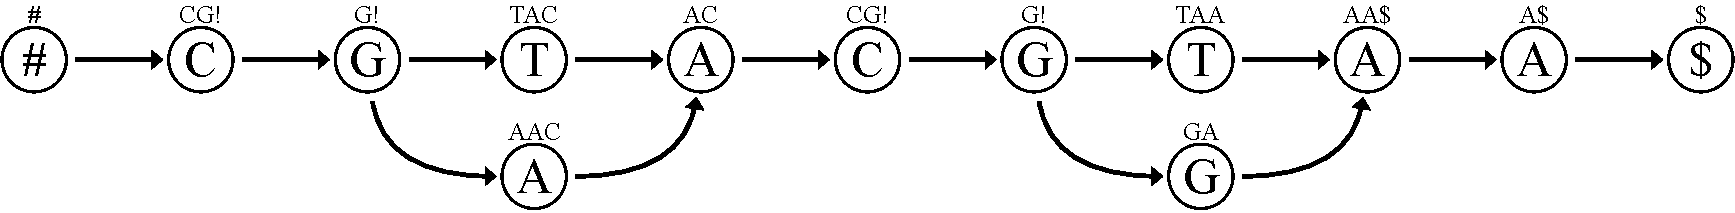
\includegraphics[width=\textwidth]{evo_gml_rev_det_but_not_prev_sort.pdf}
\caption[Reverse deterministic graph that is not prefix sorted]{Reverse deterministic graph that is not prefix sorted. Among others, the two nodes with label “C” share the same prefix.} \label{fig:evo_gml_rev_det_but_not_prev_sort}
\end{figure}
If none of the nodes in the graph had more than one outgoing edge, then the graph 
would already be prefix sorted, as every prefix would end with the dollar sign 
and have this dollar sign in a different position than any of the other prefixes would. 
However, as the nodes in the graph we consider can actually have several outgoing edges, 
it is possible that they lead to nodes which have different labels. In this case, 
we write a special character such as the exclamation point at the character in the prefix, 
to note that this character can not be unambiguously determined. \\
The process of achieving a prefix sorted graph is therefore based on iterating through 
the nodes and reducing the amount of 
prefixes which end on exclamation points, as can be seen in algorithm~\ref{alg:workOnAutomatonPrefixes}. 
\begin{algorithm}
\caption[Prefix sorting a graph]{Prefix sorting a graph by splitting nodes with prefixes that are not unambiguously sortable.}
\label{alg:workOnAutomatonPrefixes}
\begin{algorithmic}[1]
\State $ \textrm{graph\_is\_not\_prefix\_sorted} \gets \texttt{true} $
\While{graph\_is\_not\_prefix\_sorted}
	\State $ \textrm{graph\_is\_not\_prefix\_sorted} \gets \texttt{false} $
	\ForAll {this\_node \textbf{in} graph}
		\State $ \textrm{this\_node.prefix} \gets \textrm{this\_node.label} $
	\EndFor
	\ForAll {this\_node \textbf{in} graph}
	\Comment {Check for all nodes...}
		\State $ \textrm{same\_as} \gets [ \, ] $
		\ForAll {that\_node \textbf{in} graph}
		\Comment {... if any node has the same prefix}
			\If {$ \textrm{this\_node.prefix} = \textrm{that\_node.prefix} $}
				\State \textbf{append} $ [\textrm{that\_node}] $ \textbf{to} same\_as
			\EndIf
		\EndFor
		\If {\textbf{length of} $ \textrm{same\_as} > 1 $}
			\ForAll {node \textbf{in} same\_as}
			\Comment {Iterate over nodes with the same prefix}
				\State $ \textrm{first\_node\_label} \gets \textrm{next character to append to node.prefix} $
				\If {first\_node\_label cannot be found unambiguously}
					\State split the last node whose label was added to the prefix and which
						\State \phantom{first} has more than one successor
					\State $ \textrm{graph\_is\_not\_prefix\_sorted} \gets \texttt{true} $
				\Else
					\State \textbf{append} first\_node\_label \textbf{to} node.prefix
				\EndIf
			\EndFor
		\EndIf
	\EndFor
\EndWhile
\end{algorithmic}
\end{algorithm}
In line 18 of this algorithm, a node with more than one successor is split into several nodes. 
Such a node needs to exist there, as we reach this point in the algorithm due to a prefix 
not being unambiguously constructable, and the only way for this to happen is if a node has 
several successors with different prefixes. Therefore, we must be able to find a node with 
several successors for which splitting it enables us to build longer prefixes. \\
The exact approach for splitting a node $ N $ is to replace $ N $ by as many new nodes as $ N $ has 
outgoing edges. 
Every one of the nodes replacing $ N $ has exactly one outgoing edge, leading to 
one of the successors of $ N $. 
In this fashion, every successor of $ N $ obtains one of the nodes replacing $ N $ as predecessors. 
Every one of the new nodes also obtains incoming edges to all the nodes that are predecessors of $ N $. 
Finally, every one of the nodes replacing $ N $ is given the label of $ N $. 
The process of splitting a node is shown in figure~\ref{fig:evo_fig_node_splitting}. \\
% GACCTAATG|,5,C,8;,1,AG,5 - here we did a bit of work manually; this is about the splitting of the T node,
% but the position looks better after the splitting of the C node, so we copied some arrows manually in inkscape etc.
\begin{figure}[!htb]
\centering
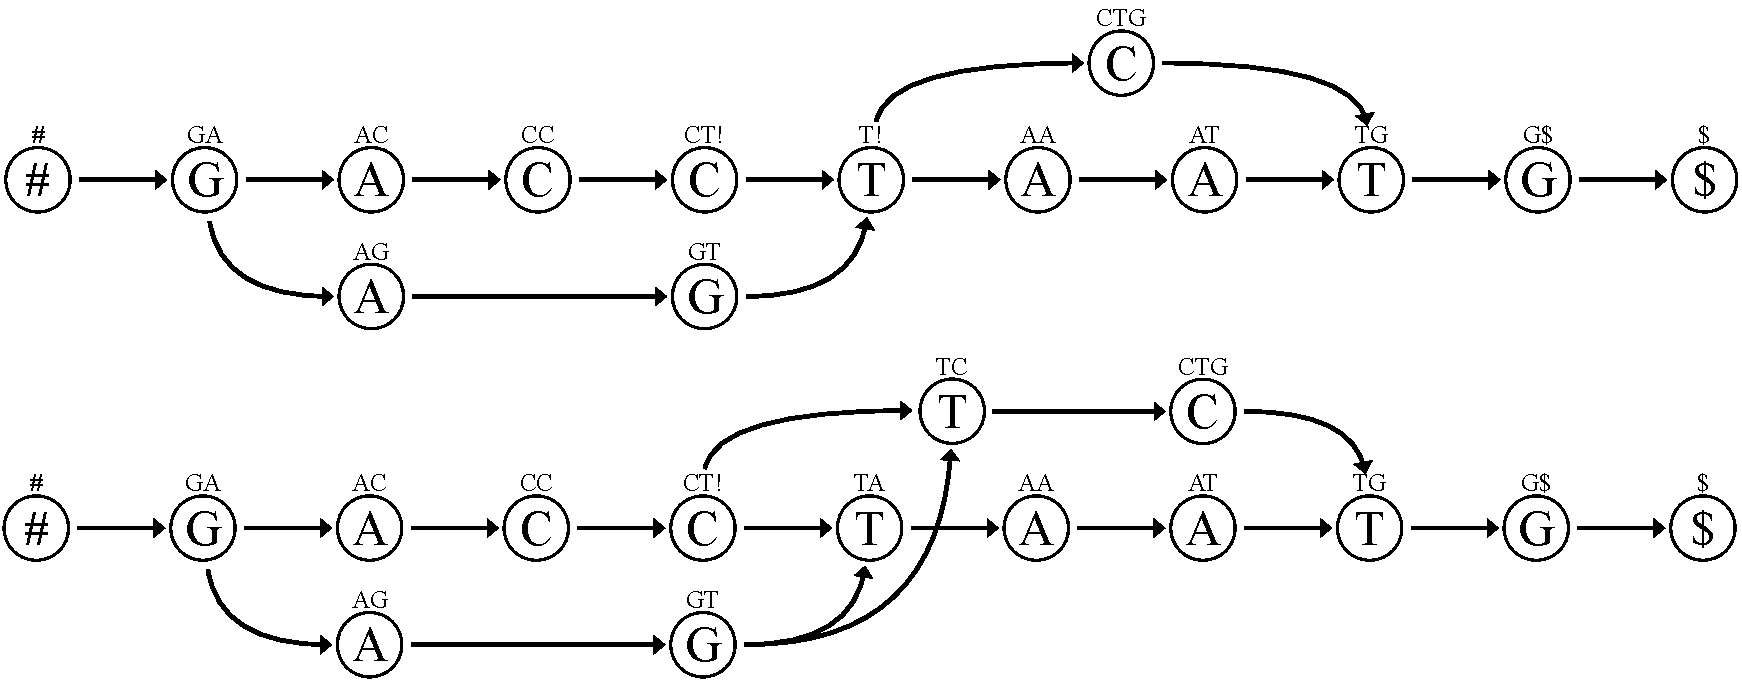
\includegraphics[width=\textwidth]{evo_fig_node_splitting.pdf}
\caption[Node splitting example]{Node splitting example. On the top, the graph is visualized before the splitting of the central node with label “T” and prefix “T!”. On the bottom, the same graph can be seen after node splitting occurred. The node has been replaced with one node with prefix “TC” and one node with prefix “TA”. Both nodes have all the incoming edges that the original node had.} \label{fig:evo_fig_node_splitting}
\end{figure}
It should be noted that we do not wish to remove all exclamation points entirely, 
as it is enough for a prefix to be so long as to be unambiguously sortable against all 
other prefixes of nodes in the graph. If a prefix is long enough to ensure this, then 
it is completely irrelevant whether it eventually ends in an exclamation point or in a dollar sign.

\subsection{Creating a Node Table}

Instead of directly generating a flat XBW table from the prefix sorted graph, 
I decided to first generate a node table. 
This is a table that shares important characteristics with a flat XBW table, 
but which is easier to understand and to use as it is closely related to the 
graph. Using the visualized graph to understand the corresponding node table 
can therefore be very helpful.

\textbf{Definition} An XBW node table is a table with rows for the BWT, 
the prefixes and the values of $ M $ and $ F $, 
representing a finite graph with each column of the table corresponding 
to exactly one node of the graph.

The columns in a node table are sorted alphabetically by the given prefix. 
For any column $ C $ representing node $ N $ in the graph, 
the value of the BWT in $ C $ represents the labels of the nodes 
preceding $ N $. 
If several nodes with different labels are preceding the node $ N $, 
then the BWT value takes on the concatenation of all these values. 
To make it clearer that a BWT containing several characters actually 
stands for any of these characters, instead of standing for the string 
formed by the characters, I decided to display BWT values containing 
more than one character separated by pipe characters, as can be 
seen in figure~\ref{fig:evo_fig_node_table_example} which is represented 
by node table~\ref{table:evo_node_table_example}. \\
% GCTGGCGAG|,3,T,5;,5,,7
{
% reduce whitespace in this table (default is 6pt I believe)
\renewcommand{\tabcolsep}{1pt}
\begin{table}[htb]
\centering
\caption[Node table corresponding to a graph]{Node table corresponding to the graph in figure~\ref{fig:evo_fig_node_table_example}.}
\begin{tabular}{ | c | c | c | c | c | c | c | c | c | c | c | c | c | c | c | c | c | c | }
\hline
G & G & G & G & A & C|G & G|T & \# & G|T & T & T & T & T & C & C & C & \$ & \textbf{BWT} \\ \hline 
\$ & A & CG & CT & G\$ & GA & GCG & GCT & GGA & GGC & GGG & TGC & TGGA & TGGC & TGGG & TT & \# & \textbf{Prefix} \\ \hline 
1 & 1 & 1 & 100 & 1 & 1 & 1 & 1 & 1 & 1 & 1 & 1 & 1 & 1 & 1 & 10 & 1 & $\boldsymbol{M}$ \\ \hline 
1 & 1 & 1 & 1 & 1 & 10 & 10 & 1 & 10 & 1 & 1 & 1 & 1 & 1 & 1 & 1 & 1 & $\boldsymbol{F}$
 \\ \hline 
\end{tabular}
\label{table:evo_node_table_example}
\end{table}
}
\begin{figure}[!htb]
\centering
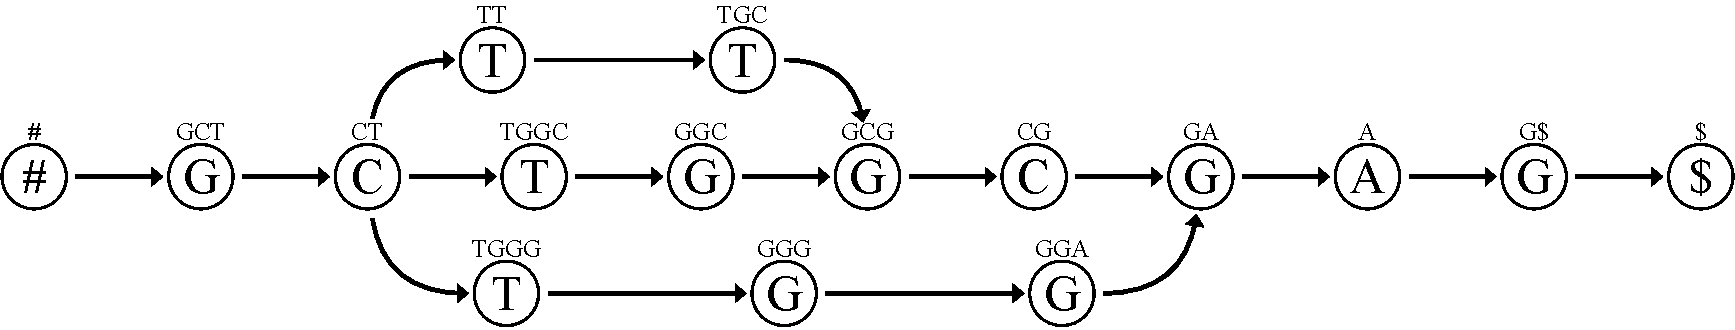
\includegraphics[width=\textwidth]{evo_fig_node_table_example.pdf}
\caption[Graph corresponding to a node table]{Graph corresponding to node table~\ref{table:evo_node_table_example}} \label{fig:evo_fig_node_table_example}
\end{figure}
The value of the prefix of $ C $ is precisely the prefix of node $ N $ in the graph, 
which is a string starting with the label of $ N $ and then containing 
the labels of the following nodes in sequence of encountering them traversing 
the graph outwards from $ N $.
The value of $ M $ is a string whose length corresponds to 
the amount of successor nodes of $ N $, or equally the amount of outgoing edges of node $ N $. 
This string always starts with the character “1” and is then followed 
by as many “0” characters as are necessary to achieve the desired length. 
Similarly, the value of $ F $ in column $ C $ is a string whose length corresponds to 
the amount of predecessor nodes of node $ N $.

\subsection{Merging Node Tables}

The main aim of the Graph Merging Library is to provide algorithms 
to merge and fuse flat XBW tables. 
However, working with flat XBW tables directly is rather cumbersome, 
and it can therefore help to first investigate the simpler case 
of merging two node tables.

% Algorithm for Merging Node Tables (function GML.merge_BWTs_advanced()):
%
% find last letter of DH_1 and first letter of DH_2
% > yepp, this is truly the label of the node BEFORE $ / the label of the node AFTER #,
%   so this assumes that there is only one edge into $ and only one edge out of #!
%
% add origin to H_1 and H_2
% concatenate H_1 and H_2 as H_12
% replace $ having origin 0 with $#firstLetterH_2 within prefixes
% ...

\subsection{Creating a Flat Table}

Having understood how merging several node tables works, we can now 
carry on with the actual flat XBW tables. 
Encoding the same graphs both as flat XBW tables and as node tables 
shows that flat XBW tables are much smaller and therefore easier to store. 
The biggest differences between the two kinds of tables, 
which can both be used to encode genomic graphs, 
are that flat tables do not contain the potentially enormously big prefix cells 
of node tables, and that flat tables do not require any overhead to 
keep track of column boundaries within a row. 
While node tables can contain strings of various sizes in all their cells, 
flat tables contain exactly one character in each cell, such that 
an entire table row can be stored as string without losing information 
about the cell boundaries. \\
This smaller size comes at the cost of simplicity. 
Within a node table, each column clearly corresponds to a node within the graph, 
and a simple manual inspection of the table can lead to various insights into the graph. 
In a flat table however, not every column describes and entire node within the graph, 
as some columns only describe parts of nodes, as e.g. a node with several predecessors 
can have information about its BWT spread across several columns in the flat table. 
In addition to that, we should not even think about whole columns in the flat table 
necessarily, as we need the $ M $ and $ F $ rows to 
find the corresponding cells across different rows, which are not necessarily located in the same columns.

To convert an XBW node table into a flat table, we need to convert the data which is now in the format of a 
node table into a flat one, a process which can be seen in 
tables~\ref{table:evo_node_to_flat_node} and \ref{table:evo_node_to_flat_flat}. 
% GATAATG|,3,C,6;,1,AG,3
{
% reduce whitespace in this table (default is 6pt I believe)
\renewcommand{\tabcolsep}{5pt}
\begin{table}[htb]
\centering
\caption[XBW node table before conversion to flat table]{XBW node table before conversion to flat table. 
Table~\ref{table:evo_node_to_flat_flat} shows the corresponding flat table.}
\begin{tabular}{ | c | c | c | c | c | c | c | c | c | c | c | c | c | c | c | }
\hline
G & T & G & G & G & A & T & T & \# & A & A|G & A|G & A|C & \$ & \textbf{BWT} \\ \hline 
\$ & AA & AG & ATA & ATC & ATG & C & G\$ & GA & GT & TA & TC & TG & \# & \textbf{Prefix} \\ \hline 
1 & 1 & 1 & 1 & 1 & 1 & 1 & 1 & 100 & 10 & 1 & 1 & 1 & 1 & $\boldsymbol{M}$ \\ \hline 
1 & 1 & 1 & 1 & 1 & 1 & 1 & 1 & 1 & 1 & 10 & 10 & 10 & 1 & $\boldsymbol{F}$ \\ \hline 
\end{tabular}
\label{table:evo_node_to_flat_node}
\end{table}
}
\begin{table}[htb]
\centering
\caption[Flat XBW table after conversion from node table]{Flat XBW table after conversion from node table. 
Table~\ref{table:evo_node_to_flat_node} shows the corresponding node table.}
\begin{tabular}{ | c | c | c | c | c | c | c | c | c | c | c | c | c | c | c | c | c | c | }
\hline
G & T & G & G & G & A & T & T & \# & A & A & G & A & G & A & C & \$ & \textbf{BWT} \\ \hline 
\$ & A & A & A & A & A & C & G & G & G & G & G & G & T & T & T & \# & \textbf{FC} \\ \hline 
1 & 1 & 1 & 1 & 1 & 1 & 1 & 1 & 1 & 0 & 0 & 1 & 0 & 1 & 1 & 1 & 1 & $\boldsymbol{M}$ \\ \hline 
1 & 1 & 1 & 1 & 1 & 1 & 1 & 1 & 1 & 1 & 1 & 0 & 1 & 0 & 1 & 0 & 1 & $\boldsymbol{F}$ \\ \hline
\end{tabular}
\label{table:evo_node_to_flat_flat}
\end{table}
For the BWT, $ M $ and $ F $ rows, the process is exactly the same. 
We join all the cells together to achieve one string containing the entire 
row, and then split this row in between every character. 
If there were pipe characters in between some of the characters, such as 
for visualization purposes within the BWT cells, then we omit them in this process. \\
The process for the prefixes is a little bit different, as the flat XBW table does 
not contain the whole prefixes due to their immense size. 
The flat XBW table can however be thought of as containing FC, the first column data (where 
the first column refers to the first column of the alphabetically sorted cyclic rotations, 
not to the first column of this table.) 
As the FC field corresponds to the label of the node, and as the prefixes in the node table 
begin with the labels of their respective nodes, the two rows are intimately linked 
and the FC row can be constructed from the prefixes in the node table. 
For the construction of the FC row, it is also necessary to consider the amount of 
outgoing edges of a node, which is encoded in $ M $. 
In total, to generate the FC row in the flat table based on the prefix and $ M $ rows in the 
node table, we start with an empty string for FC and iterate through the prefixes in the node table. 
For each prefix, we read out the first character of that prefix. 
We then add this first character as often to FC, as the contents of the $ M $ cell 
in the corresponding column are long. So if the value of $ M $ is 100, 
then the first character of that prefix needs to be added three times to FC. \\
Having constructed the BWT, FC, $ M $ and $ F $ rows from the original node table, 
we have now created a flat XBW table which represents the same graph that was represented 
by the original table.

\subsection{Working on a Flat Table}

Before considering the rather challenging problem of merging several flat XBW tables, 
we should first investigate how work within such flat tables can be performed in general. 
In particular, it is helpful to understand how 
the functions LF and $ \Psi $ can be used to find the predecessors and successors 
of nodes, respectively.

\subsection{Merging Flat Tables}

The merging of flat XBW tables is in principle similar to the merging of node tables. 
We again iterate over all nodes of all involved graphs and construct a new table 
based on them. 
However, a big difference to the merging of the node tables is that we no longer have 
a data structure available to store the computed prefixes of all columns. 
This is intentional, as storing all of these prefixes in memory would be prohibitive 
in a real-world scenario. The implication of not having the prefixes readily available 
are that we can no longer keep track of problematic nodes that easily. 
We also cannot merge the separate tables together as they are and work on the node splitting to expand the prefixes 
after the merge, as the flat XBW format relies heavily on the ordering on the columns. 
We simply cannot guarantee that we will order the columns correctly 
if we do not have expanded prefixes in the first place. \\
I therefore decided to implement the merging of flat XBW tables in two steps, 
with the first being an iteration over all columns of the tables that are supposed to be merged, 
with the aim of determining which prefixes will need to be expanded. The corresponding nodes are 
split and the prefixes recalculated until no further node splitting will be necessary when the actual 
merge occurs. \\
The second step is then to carry out the merging. This in itself is complicated by the fact 
that in flat XBW tables, entire columns do not necessarily form a union. That is, 
in the node table, each column consisting of an entry in the BWT, a prefix, and values for $ M $ and $ F $, 
represents one node in the graph, and can not be taken apart. 
However, in the flat XBW table, column do not form such a union. 
Instead, an $ F $ value of 0 shows that the BWT of this column forms a union with the BWT of the column to the left, 
and an $ M $ value of 0 shows that the first column value of this column forms a union 
with the first column value of the column to the left.

% TODO :: add algorithm!

\subsection{Fusing Instead of Merging}
\label{sec:fusing_instead_of_merging}

As shown in the previous section, merging flat XBW tables is rather complex. 
It requires a lot of computation and due to a lot of node splitting 
necessary to ensure unambiguously sortable prefixes along the entire merged 
graph can result in large amounts of node splitting. This leads to an increase 
in file size as opposed to the total file size of the individual graphs that are 
merged. \\
To explore how these problems might be avoided, 
I decided to implement another way to combining several flat XBW tables. 
In this way, consecutive graphs encoded as flat XBW tables are fused together on their ends, 
meaning that the dollar sign node of one graph is connected with the hash tag node of the next. 
This connection is not directly achieved within the data structure itself, 
but it is instead performed by the program working on the data structure, 
which in itself just contains several completely regular flat XBW tables with 
one hash tag and one dollar sign node each.

Implementing the fusing behaviour is not particularly difficult, 
as the only new occurrence to look out for is a possible spillover in which 
we leave one graph and move on to the next. In that event, the program working 
on the fused XBW data structure needs to automatically jump over the hash tag and dollar sign nodes, 
as internal hash tag and dollar sign nodes should not be accessible to the outside.

% TODO :: add more!

% TODO :: maybe we could add a picture of how two graphs are fused together on the ends?
% and show how much work would be involved in merging - that is, making the stuff prefix
% sorted after fusing - while all that can be avoided in simply letting it be that?

\chapter{Results}
% unsere Ergebnisse
%
% ====================================================================================================================================
%                                                                                                                              RESULTS
% ====================================================================================================================================

In this thesis, existing graph reference approaches have been compared 
and new algorithms have been implemented to help the community effort 
of starting to use reference graphs more widely.

\section{Formats for Genomic Graphs}

I tried out different formats in the course of this thesis, 
and noticed that indeed some do seem more appropriate for representing genomic graphs than others. \\
Surprisingly, implementing an algorithm to open a file in the seemingly simple bubble format was actually 
not easier than implementing more advanced formats like FASTG, GFA and GML.

I also noticed that none of the considered formats currently offer inbuilt compression techniques. 
Changing this however would not be very difficult. Especially in the FFX format, 
which mainly contains a BWT and two bit-vectors for each data block, 
a rather simple compression method would be to save both the BWT and the bit-vectors 
using run-length encoding. 
% TODO :: insert figure of FFX with run-length encoding switched on
Such an approach would still keep the format simple enough to be implemented in various 
tools in the future, while offering a significant file size reduction. 
This reduction is especially strong when data is encoded that contains long linear sections 
interspersed with some short graphs, as both of bit-vectors will then 
contain very long runs. \\
It is of course also possible to create even more compressed versions 
of the different formats by not saving the contents of the files as ASCII text, 
but instead as bitwise data structures that can e.g. represent each of the nucleotides A, C, G and T with 
just two bits.

\section{Merging XBWs}

Using the Graph Merging Library, I have explored several ways to merge XBWs. 
As could be expected, merging two node tables is a much simpler process than merging two flat tables, 
as a node table is much less compressed, and working on it is simpler in general. 
The node table not being as compressed as a flat table though means 
that it would not be practical in a real-life scenario to merge these kinds of tables.

However, even when choosing to merge two flat XBW tables, 
the merge result can become unnecessarily large.

% TODO :: insert picture - a graph, another, and then merged soooo big as the thing is split and split and split

\section{Fusing XBWs Instead of Merging Them}

When merging flat XBW tables together, it is common that node splitting 
will result in a merged graph with a size larger than the total size of the 
original graphs. 
Fusing flat XBW tables together omits the need for this increased file size, 
which not only makes it easier to store the data, but also means that working on 
it is quicker as less data means that fewer operations are necessary to construct 
distinct prefixes, to traverse all possible paths, and so one.

However, fusing flat XBW tables also has downsides. 
One of them is related to indexing. 
When working with a merged graph, every column in the graph has a clear integer index, 
so that locations within the entire graph can simply be referred to with a single integer value. 
With a fused XBW however, in addition to specifying a column within the table, 
it also needs to specified which table is addressed, necessitating pairs of integers. 
If particularly large list of locations needs to be created, this difference of two integers instead of one 
could become problematic. \\
Also, it is algorithmically more complex to work with fused graphs, as every 
algorithm working on the graph needs to be prepared to handle spillover scenarios, 
in which the end of one of the fused graphs is reached and the execution needs to continue 
within the next graph. \\
These spillover scenarios might also severely limit the otherwise seemingly 
great possibilities for splitting the computation of fused graphs across different 
cores in a distributed system. 
If each processor core is supposed to work on exactly one graph, 
but spillovers are happening frequently, then some cores would stop having work 
to do as no further work would be going on within their data block, 
while others would have to do twice as much work by caring for their 
own work before working on the activity that spilled over from the other data block. \\
Finally, setting up such a system in the first place might be difficult to do, 
as a fused file would most likely contain large areas of linear data, 
fused together with short blocks of graph data. Therefore, assigning one 
data block to one core and letting it perform work in this straightforward fashion 
would lead some cores to have to do much more work than the others, ultimately 
leading to many idle cores waiting for a few to finish which were given much more work 
to do in the first place. This is obviously not desirable in a multi-core system, 
in which ideally all the processor cores should be working for the same time 
and then be done together in the quickest time possible.

However, at least some of these problems could be overcome fairly easily. 
Spillover scenarios as an example, which with a naive 
implementation would possibly lead to some cores having no work to do 
after a spillover happened while other cores would have to do twice as much, 
could be avoided by giving the cores access not only to their own data blocks, 
but also to the data in the surrounding blocks. Then each core could handle 
and complete its own spillovers, without requesting assistance from its neighbours.

\chapter{Conclusions}
% AKA: summarize our data and compare with methodology to see if we fulfilled what we set out to do
%
% ====================================================================================================================================
%                                                                                                                          CONCLUSIONS
% ====================================================================================================================================

Aligning reads from human DNA to graph references rather than to string reference sequences 
still offers many interesting problems. 
However, the first steps on the way to using reference graphs in real-world applications have been made.

\section{Discussion}

Despite a lot of work already having been done to explore 
ways of using genomic graphs within the field of human DNA analysis, 
using reference graphs rather than reference strings still 
is a difficult proposition and only few tools exist that incorporate 
such methods. 
It could therefore be argued that the known advantages of using reference 
graphs do not outweigh the tremendous difficulties that have to 
be overcome in order to be able to use them on a large scale. \\
After all, the reason why reference graphs are proposed to be used 
rather than reference strings is to improve alignment results 
and to simplify the calling of known variants. 
But at least in the beginning when only small local graphs are incorporated 
into largely linear references, the improvements are likely to be very slim. 
Likewise, it could be questioned whether simplifying the calling of variants really 
justifies complicating matters so much in general by the introduction of 
these new graph structures.

However, I would argue that in the long run, reference graphs will come to be used. 
With every new individual DNA that is constructed, more insight is gained into 
variations which could be quite common among populations. 
Discarding all of that data in favour of a simpler but ultimately flawed approach 
will not work forever, as over time better alignment results will come to be expected. \\
Therefore, it seems inevitable to work on reference graphs eventually, 
and it seems only logical to start that work as soon as possible, rather than investing 
more time and resources into improving current alignment tools which are likely to be drastically 
modified to incorporate reference graphs in the future anyway.

\section{Future Work}
% AKA: Possibilities for SOMEONE ELSE to make it even better

There still remains a lot of future work to be undertaken to actually use 
the already existing and the here newly proposed algorithms in real-world 
tools of the analysis pipeline. 
As various different tools are in use for specific problems, no one implementation 
is likely to achieve this. Instead, the community at large needs to start 
incorporating the ideas of using graph data rather than sequential data into 
more and more of the existing tools.

\bibliography{thesisreferences}

\appendix
\renewcommand{\chaptername}{Appendix}
\chapter{Appendix}
%
% ====================================================================================================================================
%                                                                                                                             APPENDIX
% ====================================================================================================================================

\section{Resources and Licensing}

Publicly available genomic datasets as well as automatically generated data were used 
to implement the new graph reference approaches and to analyse the results of the implementations.

Recently, there has been a push towards implementing more open source scripts 
and programs within the scope of bioinformatics \citep{MANIFESTO}. \\
All of the software developed while working on this thesis 
is open source and distributed under the terms of 
the Creative Commons Attribution Non-Commercial License 
(\url{http://creativecommons.org/licenses/by-nc/3.0/}), 
% TODO :: check (ask someone?) if this is the correct license to be used here
which permits non-commercial re-use, distribution, and reproduction in any medium, 
provided the original work is properly cited. 
For commercial re-use, please contact \url{moyaccercchi@hotmail.de}. \\
The source codes together with the newest version of the thesis itself can be accessed at \url{http://tomschiller.de/graphalign}.
% 
% TODO :: add stuff to the appendix!

%
%
% don't let any reference remain unused!
% \phantom{
% References that are so far not referred to anywhere else in the text:
% }
%
%

\end{document}

% TODO :: check if all our lists are in the following format
%
% ullet list
% Hér á eftir er dæmi um upptalningarlista. Listinn má vera þéttari, 
% þ.e. að aðeins sé 0 pt bil á milli atriða, en þó skal hafa 12 pt bil á undan fyrsta atriði listans.
% \begin{itemize}
%  \item Númer 1
%  \item Númer 2
%  \item Númer 3
% \end{itemize}
% Ef fyrsta lína eftir upptalningu er framhald sömu málsgreinar og fyrir ofan 
% skal ekki setja inn viðbótarloftun (eða ef inndráttur er notaður, 
% skal ekki nota inndrátt á slíkri línu).

% TODO :: check if all our figures and tables are in the following format
% 
% \chapter{Figures and tables}
% { \color{red} Þessi kafli sýnir dæmi um notkun mynda, taflna og vísun í þær. }
% 
% \section{Figures}
% { \color{red} Myndatexti skal staðsetja undir myndum og skrifast með skáletri.
% Setja skal auða aukalínu fyrir ofan myndir.
% \begin{figure}[!htb]
% \centering
% 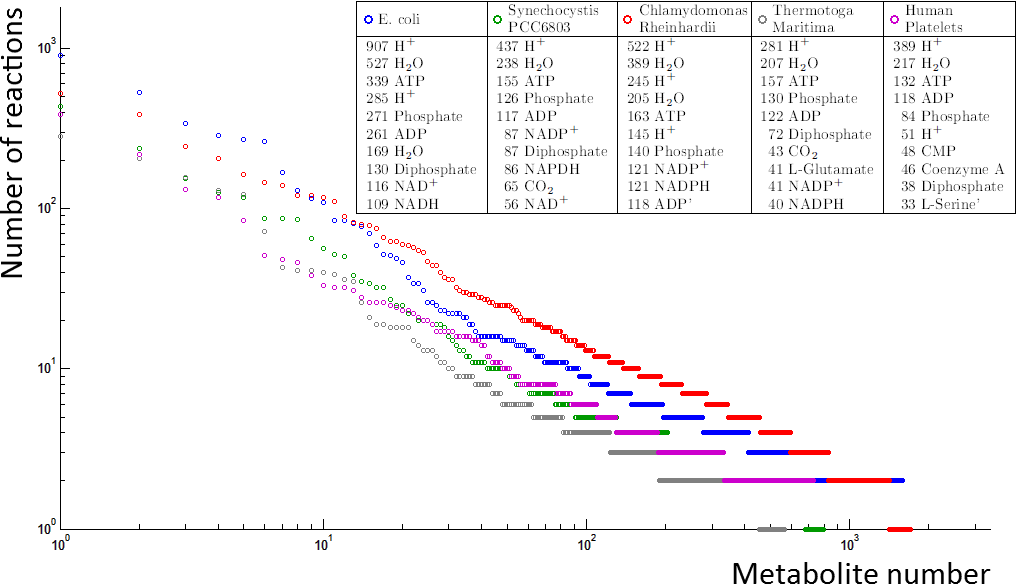
\includegraphics[width=0.47\textwidth]{evo_example_pic.png}
% \caption[Dæmi um myndatexta (fyrir neðan mynd).]{Dæmi um myndatexta (fyrir neðan mynd)} \label{fig:Example Pic}
% \end{figure}
% Mikilvægt er að skilgreina myndir með ,,paragraph format”: “keep with next” til að rjúfa 
% ekki tengsl á milli myndar og myndtexta. Mynd má vera miðjuð og skal þá einnig miðja myndartextann. 
% Letur innan myndar skal vera í steinskrift (sans serif), t.d. Verdana, og ekki minna en 10 pt. 
% Tryggið að letur, tákn og línur sjáist skýrt eftir útprentun.
% 
% Hægt er að láta númera og merkja myndir sjálfvirkt með því 
% að gera Insert – Reference – Caption – Mynd eða Tafla. 
% Varist að velja hyperlink. 
% 
% Vísa má í mynd með því að velja Insert – Reference – Cross-Reference – Mynd eða Tafla. 
% Varist að velja hyperlink og veljið að eins Label og Number. 
% T.d. sjá þessa tilvísun í Mynd 3.1 sem dæmi. }
% 
% \section{Tables}
% { \color{red} Einnig má númera töflur sjálfkrafa svipað og myndir. 
% Nota skal skáletur í töflutitil. Textinn skal standa fyrir ofan töflu og fylgja töflunni. 
% Ekki nota tvöfalt línubil eða hafa space before í töflum. 
% Meginreglan við töflugerð er að hafa þær einfaldar og eins fá strik og mögulegt er. 
% Tafla má vera miðjuð á blaðsíðu og skal þá láta töflutitil byrja við vinstri brún töflu.
% 
% \begin{table}[htb]
% \centering
% \caption{Dæmi um töflutexta (fyrir ofan töflu).}
%      \sffamily \begin{tabularx}{1.0\textwidth}{ p{5cm}  p{5cm}  p{5cm} }
%     \hline
%    \textbf{Taflan} \hfill & \textbf{Er} \hfill & \textbf{Eins} \\ \hline
%     Og & Hún & gæti\\
%     Litið & Út & í ritgerð\\ \hline
%     \end{tabularx} \normalfont
% \label{table:Emissivity}
% \end{table}
% 
% Almennt skal ekki nota loftun fyrir neðan texta í töflu, og stylla loftun fyrir neðan á 0 pt.
% Mikilvægt er að skilgreina töflutexta með ,,format paragraph: keep with next og keep lines together” til að 
% rjúfa ekki tengsl á milli töflutexta og töflu. 
% Ef tafla er mjög löng má kljúfa hana á milli blaðsíðna og þá verður 
% að setja (\textit{Framhald}) í aukalínu beint fyrir neðan töfluna, 
% hægri stillt við hægri brún töflu.
% 
% Dæmi um sjálfvirka tilvísun í töflu, bara nota Label and Number, 
% ekki nota hyperlink eða caption text. T.d. Tafla 3.1 sýnir dæmi um töflu. }
